% Arquivo LaTeX de exemplo de dissertação/tese a ser apresentada à CPG do IME-USP
%
% Criação: Jesús P. Mena-Chalco
% Revisão: Fabio Kon e Paulo Feofiloff
% Adaptação para UTF8, biblatex e outras melhorias: Nelson Lago
%
% Except where otherwise indicated, these files are distributed under
% the MIT Licence. The example text, which includes the tutorial and
% examples as well as the explanatory comments in the source, are
% available under the Creative Commons Attribution International
% Licence, v4.0 (CC-BY 4.0) - https://creativecommons.org/licenses/by/4.0/


%%%%%%%%%%%%%%%%%%%%%%%%%%%%%%%%%%%%%%%%%%%%%%%%%%%%%%%%%%%%%%%%%%%%%%%%%%%%%%%%
%%%%%%%%%%%%%%%%%%%%%%%%%%%%%%% PREÂMBULO LaTeX %%%%%%%%%%%%%%%%%%%%%%%%%%%%%%%%
%%%%%%%%%%%%%%%%%%%%%%%%%%%%%%%%%%%%%%%%%%%%%%%%%%%%%%%%%%%%%%%%%%%%%%%%%%%%%%%%
\documentclass[a4paper,12pt,twoside,english,brazilian]{book}

\usepackage{imegoodies}
\usepackage[thesis]{imelooks}
\graphicspath{{figures/},{logos/},{images/}}
\babeltags{br = brazilian, en = english}


%%%%%%%%%%%%%%%%%%%%%%%%%%%%%%%%%%%%%%%%%%%%%%%%%%%%%%%%%%%%%%%%%%%%%%%%%%%%%%%%
%%%%%%%%%%%%%%%%%%%%%%%%%%%%%%%%%% METADADOS %%%%%%%%%%%%%%%%%%%%%%%%%%%%%%%%%%%
%%%%%%%%%%%%%%%%%%%%%%%%%%%%%%%%%%%%%%%%%%%%%%%%%%%%%%%%%%%%%%%%%%%%%%%%%%%%%%%%
\addbibresource{main.bib}
\nocite{*}

\babelhyphenation{documentclass latexmk soft-ware clsguide}

\title{Aplicações de Computação Gráfica na construção de visuais estilizados, level design e jogabilidade para um jogo 3D}
\translatedtitle{Applications of Computer Graphics in the creation of stylized visuals, level design, and gameplay for a 3D game}

\author{Diogo Ribeiro de Faria, Adriano Elias Andrade, Guilherme Henrique Vasconcelos da Cunha}

\orientador{Dr. Wilson Kazuo Mizutani}

\tipotese{
  tcc,
  programa={Ciência da Computação},
}

\defesa{
  local={São Paulo},
  data={2026-11-30},
}

\direitos{CC-BY}

\fichacatalografica{
% \noindent Para gerar a ficha catalográfica, acesse \url{https://fc.ime.usp.br},
}


%%%%%%%%%%%%%%%%%%%%%%%%%%%%%%%%%%%%%%%%%%%%%%%%%%%%%%%%%%%%%%%%%%%%%%%%%%%%%%%%
%%%%%%%%%%%%%%%%%%%%%%%%%%%%%%%%%% CONTEÚDO %%%%%%%%%%%%%%%%%%%%%%%%%%%%%%%%%%%%
%%%%%%%%%%%%%%%%%%%%%%%%%%%%%%%%%%%%%%%%%%%%%%%%%%%%%%%%%%%%%%%%%%%%%%%%%%%%%%%%
\begin{document}

%%%%%%%%%%%%%%%%%%%%%%%%%%% CAPA E PÁGINAS INICIAIS %%%%%%%%%%%%%%%%%%%%%%%%%%%%
\frontmatter

\pagestyle{plain}

\onehalfspacing % Espaçamento 1,5 na capa e páginas iniciais

\maketitle

%%%%%%%%%%%%%%%% DEDICATÓRIA, AGRADECIMENTOS, RESUMO/ABSTRACT %%%%%%%%%%%%%%%%%%
\begin{dedicatoria}

\end{dedicatoria}

\pagenumbering{roman}

\chapter*{Agradecimentos}
\epigrafe{Do. Or do not. There is no try.}{Mestre Yoda}

Texto texto texto texto texto texto texto texto texto texto texto texto texto
texto texto texto texto texto texto texto texto texto texto texto texto texto
texto texto texto texto texto texto texto texto texto texto texto texto texto
texto texto texto texto. Texto opcional.

%!TeX root=../main.tex

\palavraschave{Palavra-chave1, Palavra-chave2, Palavra-chave3}
\keywords{Keyword1,Keyword2,Keyword3}

\resumo{
Elemento obrigatório, constituído de uma sequência de frases concisas e
objetivas, em forma de texto. Deve apresentar os objetivos, métodos empregados,
resultados e conclusões. O resumo deve ser redigido em parágrafo único, conter
no máximo 500 palavras e ser seguido dos termos representativos do conteúdo do
trabalho (palavras-chave). Deve ser precedido da referência do documento.
Texto texto texto texto texto texto texto texto texto texto texto texto texto
texto texto texto texto texto texto texto texto texto texto texto texto texto
texto texto texto texto texto texto texto texto texto texto texto texto texto
texto texto texto texto texto texto texto texto texto texto texto texto texto
texto texto texto texto texto texto texto texto texto texto texto texto texto
texto texto texto texto texto texto texto texto.
Texto texto texto texto texto texto texto texto texto texto texto texto texto
texto texto texto texto texto texto texto texto texto texto texto texto texto
texto texto texto texto texto texto texto texto texto texto texto texto texto
texto texto texto texto texto texto texto texto texto texto texto texto texto
texto texto.
}

\abstract{
Elemento obrigatório, elaborado com as mesmas características do resumo em
língua portuguesa. De acordo com o Regimento da Pós-Graduação da USP (Artigo
99), deve ser redigido em inglês para fins de divulgação. É uma boa ideia usar
o sítio \url{www.grammarly.com} na preparação de textos em inglês.
Text text text text text text text text text text text text text text text text
text text text text text text text text text text text text text text text text
text text text text text text text text text text text text text text text text
text text text text text text text text text text text text.
Text text text text text text text text text text text text text text text text
text text text text text text text text text text text text text text text text
text text text.
}


\tableofcontents

% Referências indiretas para o índice remissivo
% \index{Inglês|see{Língua estrangeira}}

%%%%%%%%%%%%%%%%%%%%%%%%%%%%%%%% CAPÍTULOS %%%%%%%%%%%%%%%%%%%%%%%%%%%%%%%%%%%%%
\mainmatter

\pagestyle{mainmatter}

\singlespacing

\pagestyle{unnumberedchapter}
%!TeX root=../main.tex

\chapter{Introdução}
\label{cap:introducao}

Em 20 de Abril de 1951 começa oficialmente a operação do \textit{Whirlwind I}, o primeiro computador
a conseguir exibir imagens gráficas em um monitor de tubo de raios catódicos em tempo real,
permitindo interação com o usuário. Desenvolvido por Jay Forrester e Robert Everett no
MIT (\textit{Massachusetts Institute of Technology}) e financiado pelas Forças Armadas dos Estados
Unidos, este computador tinha como objetivo inicial ser um simulador de voo analógico, mas
que eventualmente evoluiu para um sistema eletrônico digital. Embora desenvolvido para este
propósito, este computador já contava com um dos primeiros jogos eletrônicos da história, o
\textit{bouncing ball game}, feito para demonstrar a simulação física de movimento de uma bola quicando.

Desde então, a computação gráfica e os jogos evoluíram lado a lado, impulsionados por uma
busca contínua pelo fotorrealismo e por uma simulação fiel do mundo real. Essa corrida
tecnológica existe até os dias de hoje, com o exemplo recente mais famoso sendo a
implementação do DLSS5 em placas de vídeo modernas, uma tecnologia que utiliza redes neurais
e algoritmos de aceleração baseados em Inteligência Artificial para renderizar iluminação em
tempo real e cenas geometricamente complexas.

No entanto, para atingir este nível de processamento, a computação gráfica foi limitada pelas
restrições de hardware ao decorrer da história. Nas décadas de 1980 e 1990, a incapacidade de
processar grandes volumes de dados em tempo real exigia soluções criativas de otimização,
sendo então consolidadas técnicas como a modelagem de baixa poligonização (\textit{low-poly}), para
uma renderização mais eficiente, e a projeção isométrica, utilizada para simular profundidade e
exibir grandes cenários tridimensionais em ambientes 2D com baixo custo de processamento.

Com o avanço tecnológico, técnicas como essas deixaram de ser requisitos técnicos e se
tornaram uma linguagem de expressão visual. Enquanto jogos de alto orçamento (\textit{AAA})
continuam perseguindo a complexidade gráfica, desenvolvedores independentes conseguem
usar desta linguagem para liberar recursos de hardware e focar em outros aspectos de seus
jogos, como um desempenho mais acessível para o público e em como os aspectos visuais
podem afetar o \textit{game design} e o \textit{level design} do projeto.

Nesse quesito, o estilo do jogo influencia diretamente o \textit{game design} --- conjunto de regras,
mecânicas e dinâmicas de interação --- e o \textit{level design}, responsável pelo planejamento
espacial, arquitetura dos ambientes e pela curva de desafio oferecida ao jogador. Para este
projeto, destaca-se em particular jogos das categorias de aventura e \textit{fast-paced}. Enquanto
jogos de aventura exigem cenários visualmente desenvolvidos que estimulem a exploração, a
navegação e a resolução de quebra-cabeças, jogos \textit{fast-paced} demandam uma movimentação
dinâmica e precisa, com respostas imediatas aos comandos do jogador.

Portanto, com a redução de detalhes em modelos \textit{low-poly} e a projeção isométrica da câmera
do jogo, é possível manipular como o jogador identifica obstáculos, trajetórias e diferentes
geometrias de cenário enquanto executa comandos, navega e enfrenta diferentes desafios.

Então, sob a perspectiva deste trabalho, a escolha destas técnicas permite a exploração das
etapas do \textit{pipeline} gráfico para aprofundar o conhecimento em \textbf{Aplicações de Computação Gráfica
na construção de visuais estilizados, \textit{level design} e jogabilidade para um jogo 3D}, por
meio da implementação de diferentes interações entre objetos e métodos de renderização de
modelos, pixels e iluminação.

\section**{Objetivos}

O objetivo deste trabalho é projetar, desenvolver e documentar um jogo eletrônico de aventura
e ação \textit{fast-paced} em perspectiva isométrica 3D, utilizando estética \textit{low-poly} pixelizada, com
foco na integração entre mecânicas de física, computação gráfica, \textit{game design} e \textit{level design}.

Para atingir este objetivo, foram estabelecidas as seguintes metas:

\begin{description}
	\item[Desenvolver a arquitetura básica de movimentação e colisão:] Implementar um sistema
	de movimentação dinâmico e responsivo (\textit{fast-paced}) focado em física, incluindo
	mecânicas de aceleração, deslize em superfícies e navegação fluida em rampas e
	obstáculos;
	\item[Estruturar o primeiro cenário (Movimentação):] Projetar desafios de \textit{level design}
	baseados em navegação avançada e mecânicas de mobilidade (\textit{parkour});
	\item[Estruturar o segundo cenário (Interação):] Implementar sistemas de manipulação e
	destruição de objetos tridimensionais do cenário, permitindo a abertura de novas rotas e
	resolução de obstáculos;
	\item[Estruturar o terceiro cenário (Iluminação):] Desenvolver quebra-cabeças e dinâmicas de
	ambiente fundamentados em técnicas de iluminação e reatividade de materiais à luz;
	\item[Implementar o confronto final e integração de mecânicas:] Projetar um combate contra
	um chefe final que exija a aplicação combinada de todas as ferramentas e mecânicas
	adquiridas ao longo dos cenários anteriores;
	\item[Aplicar técnicas de estilização no \textit{pipeline} gráfico:] Integrar os modelos \textit{low-poly}, a
	renderização pixelizada e a projeção ortográfica isométrica, mantendo a legibilidade
	espacial e o desempenho do jogo.

\end{description}

\section**{Estrutura do Texto}


%!TeX root=../main.tex

\chapter{Conceitos}
\label{cap:conceitos}

\section{Isometria}
\label{sec:isometria}

A projeção isométrica é um caso particular da projeção ortogonal que permite a representação
gráfica tridimensional em superfícies bidimensionais. Matematicamente, a isometria é
caracterizada pelo alinhamento dos eixos coordenados (\textbf{X}, \textbf{Y} e \textbf{Z}) em relação ao plano de
projeção, de modo que os ângulos formados entre a projeção de cada par de eixos sejam
exatamente iguais a 120$\degree$. Essa propriedade garante que a escala de medida permaneça
uniforme ao longo de todos os eixos, eliminando os pontos de fuga característicos da
perspectiva cônica, que é a forma como o olho humano enxerga a realidade.

\begin{figure}[H]
	\centering
	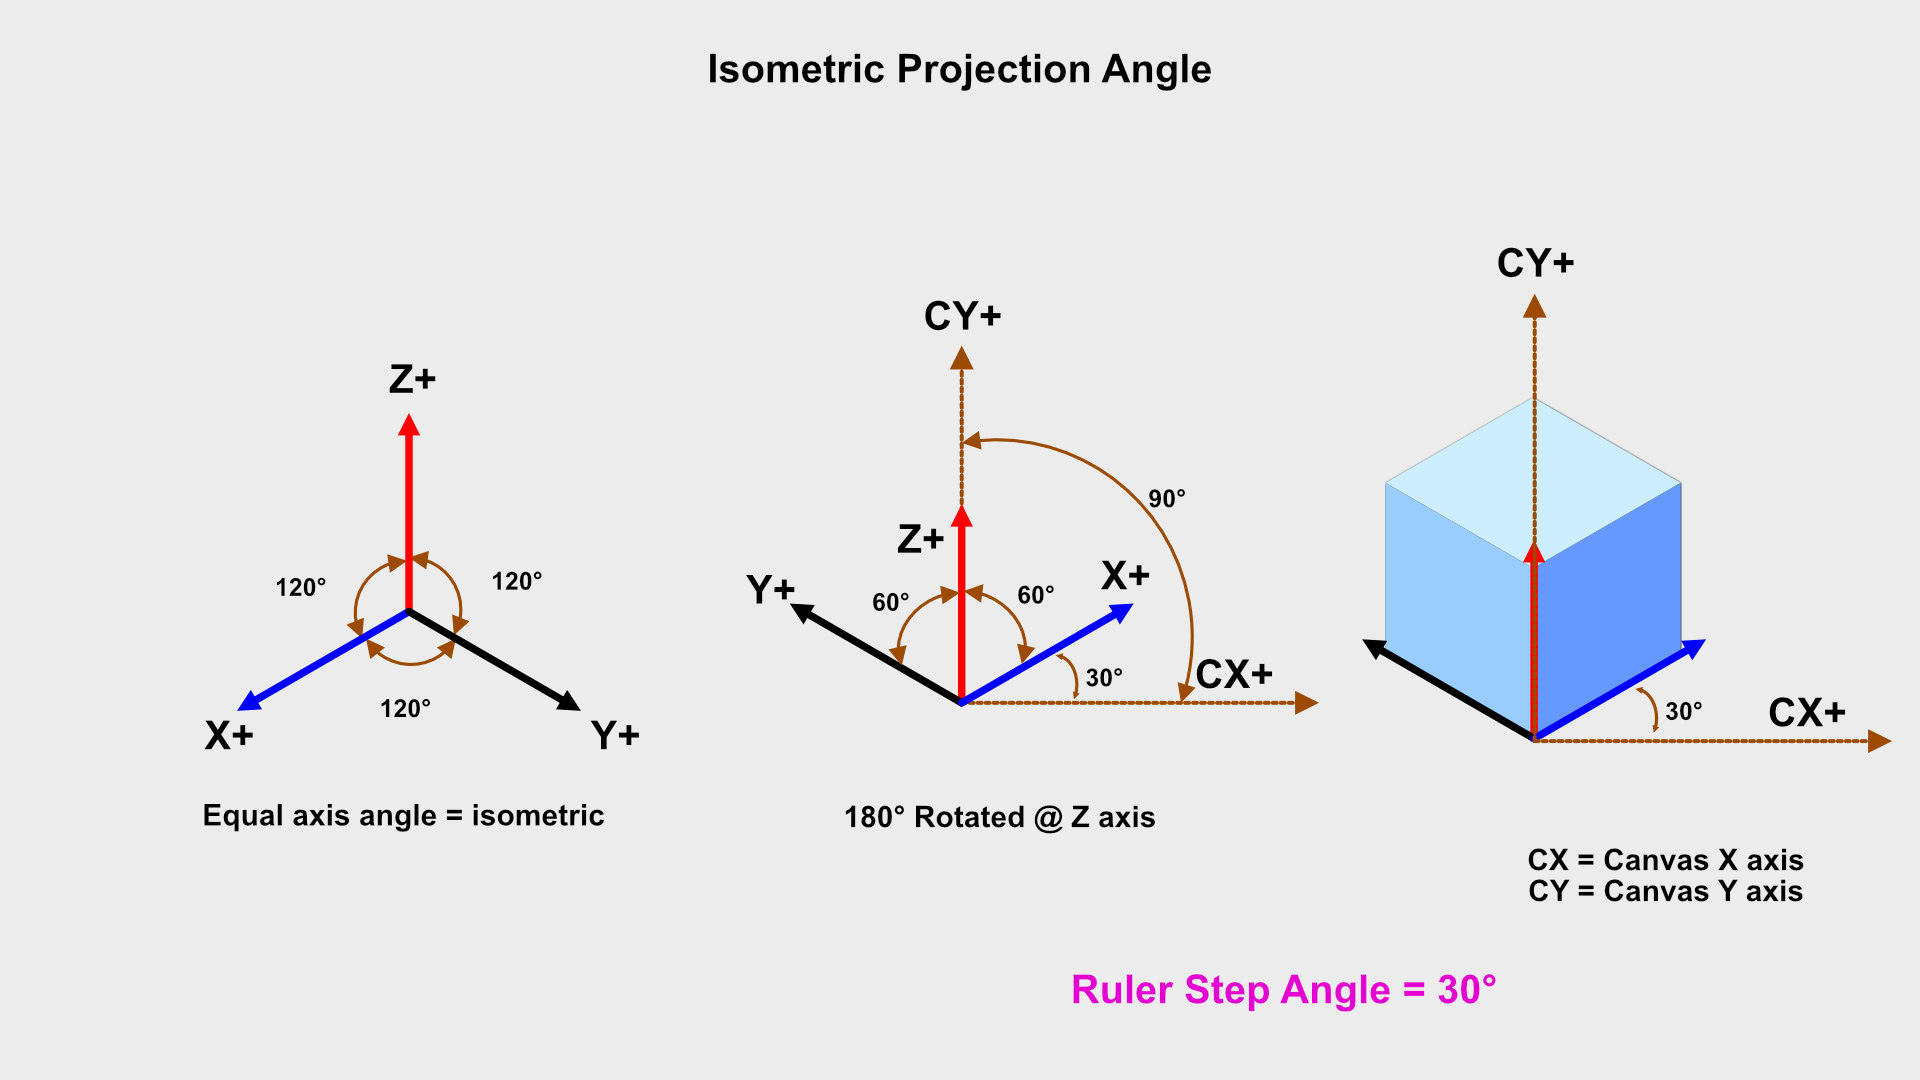
\includegraphics[width=0.7\textwidth]{isometric-120}
	\caption{Eixos X, Y e Z em uma projeção isométrica em relação ao canvas. Fonte: \cite{isometric-120}}\label{fig:isometric-120}
\end{figure}

Historicamente, o uso da perspectiva isométrica na indústria de jogos eletrônicos surgiu no
início da década de 1980 como uma solução para contornar limitações computacionais dos
hardwares da época. Antes do surgimento das unidades de processamento gráfico (GPUs)
dedicadas ao 3D em tempo real, renderizar polígonos tridimensionais complexos era inviável.
Os desenvolvedores passaram, então, a utilizar \textit{sprites} bidimensionais desenhados em ângulo
isométrico, popularizando a clássica proporção de inclinação de 2:1 em \textit{pixel art}, o que
permitia criar uma ilusão de profundidade e volume sem o custo computacional de cálculos de
perspectiva.

Todavia, esta proporção 2:1 não é uma projeção isométrica verdadeira. A projeção isométrica é um
tipo de projeção axonométrica, que é uma categoria mais ampla de projeções ortogonais (paralelas).
Nessas projeções, os ângulos entre os eixos podem variar, mas por serem projeções paralelas,
elas eliminam os pontos de fuga característicos da perspectiva cônica. A projeção axonométrica
é subdividida em três tipos:

\begin{description}
	\item[Isométrica] Caracteriza-se pela igualdade perfeita entre os ângulos formados pelos três eixos,
	cada um medindo exatamente $120^\circ$ entre si (com uma inclinação de $30^\circ$ em relação à linha
	horizontal de referência). Essa propriedade garante que a escala espacial e o fator de proporção sejam
	idênticos ao longo de todas as dimensões;
	\item[Dimétrica] Apresenta dois ângulos iguais entre a projeção dos eixos e um ângulo distinto,
	resultando em duas escalas de medição idênticas e uma terceira diferente.
	\item[Trimétrica] Todos os três ângulos entre os eixos são diferentes entre si.
\end{description}

\begin{figure}[H]
	\centering
	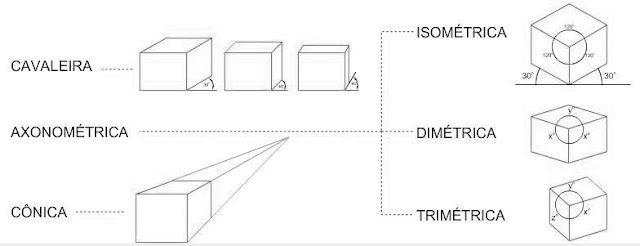
\includegraphics[width=0.8\textwidth]{axonometria}
	\caption{Tipos de perspectivas mais utilizadas. Fonte: \cite{axonometric}}\label{fig:axonometric}
\end{figure}

Ou seja, em uma perspectiva isométrica perfeita ($120^\circ$), a linha diagonal sobe a um ângulo exato
de $30^\circ$ ($\tan(30^\circ) \approx 0{,}577$). Na era da \textit{pixel art}, traçar uma linha com inclinação de $30^\circ$ era
impossível sem gerar \textit{aliasing} (serrilhamento irregular) pesado na tela. Para resolver isso, os desenvolvedores
criaram a regra prática de ``andar'' 2 \textit{pixels} na horizontal para 1 \textit{pixel} na vertical, resultando em uma inclinação de $26{,}565^\circ$
($\arctan(0{,}5) = 26{,}565^\circ$), que é a proporção 2:1. Como essa inclinação não é exatamente $30^\circ$, os ângulos entre os
eixos tornam-se aproximadamente $116{,}565^\circ$, $116{,}565^\circ$ e $126{,}87^\circ$, o que caracteriza uma projeção dimétrica, 
mas que ainda é comumente referida como isométrica na indústria de jogos eletrônicos pois a simula muito bem visualmente.

Os principais marcos durante o pioneirismo desta técnica foram os jogos \textit{Zaxxon} (1982), \textit{Ant Attack} (1983)
e \textit{Knight Lore} (1984):

\begin{description}
	\item[\textit{Zaxxon} (1982):] É um jogo de tiro espacial onde o jogador pilota uma nave em uma
	base inimiga com movimento baseado em rolagem diagonal, sendo também um dos primeiros jogos a
	exibir sombras na tela, para indicar a posição da nave em relação à superfície. Desenvolvido pela
	SEGA em 1982, é amplamente reconhecido como o primeiro jogo eletrônico a empregar a projeção
	axonométrica, que inclusive dá nome ao jogo (\textit{AXXON} vem de \textit{AXONométrica}).
	\begin{figure}[H]
		\centering
		\begin{subfigure}{0.4\textwidth}
			\centering
			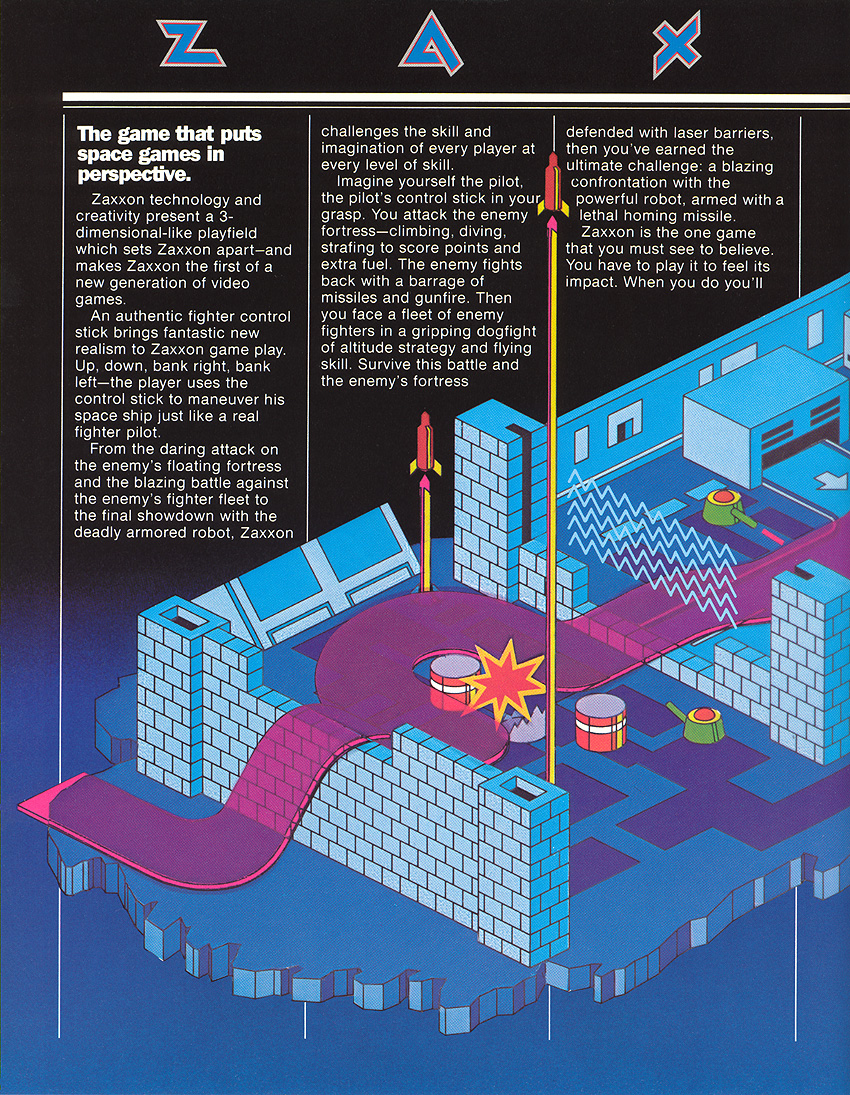
\includegraphics[width=\textwidth]{zaxxon-flyer-a}
			\label{fig:zaxxon:a}
		\end{subfigure}
		\begin{subfigure}{0.4\textwidth}
			\centering
			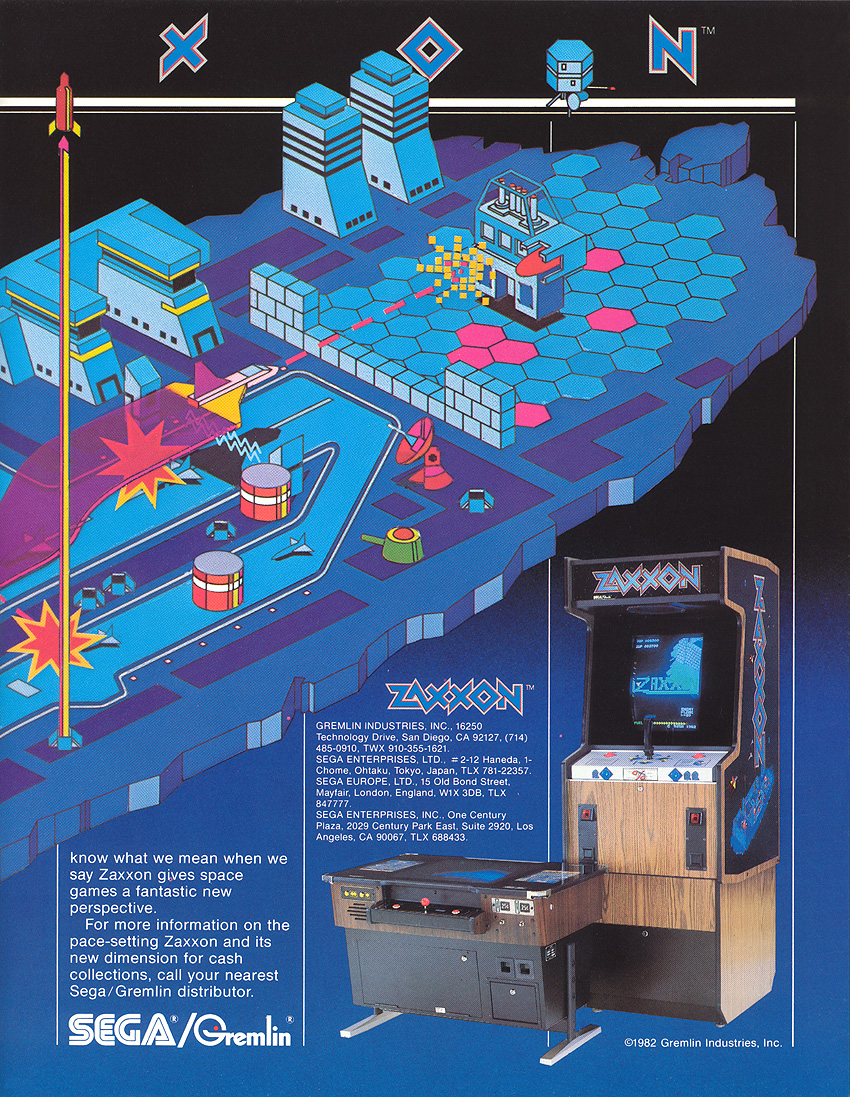
\includegraphics[width=\textwidth]{zaxxon-flyer-b}
			\label{fig:zaxxon:b}
		\end{subfigure}
		\caption{Folheto promocional de Zaxxon para Arcade. Fonte: \cite{zaxxon-flyer}}\label{fig:zaxxon}
	\end{figure}
	\item[\textit{Ant Attack} (1983):] Embora não tenha sido o primeiro jogo isométrico, foi o primeiro
	a adicionar um grau de liberdade vertical, permitindo que o jogador pudesse se mover livremente
	também para cima e para baixo, ao invés de apenas norte, sul, leste e oeste. Sendo talvez o primeiro
	jogo isométrico para computadores pessoais e também um dos primeiros a permitir que o jogador escolha
	seu gênero. Desenvolvido em 1983 por Sandy White para o ZX Spectrum, neste jogo o usuário começa
	escolhendo controlar o garoto ou a garota, então entra na cidade fortificada de Antescher para
	salvar o outro que foi capturado e imobilizado em algum lugar da cidade. A cidade é habitada por
	formigas gigantes que perseguem e mordem o jogador, cuja única forma de se defender é arremessando
	granadas que também podem machucar outros humanos. O objetivo do jogo é localizar o refém e escapar
	da cidade.
	\begin{figure}[H]
		\centering
		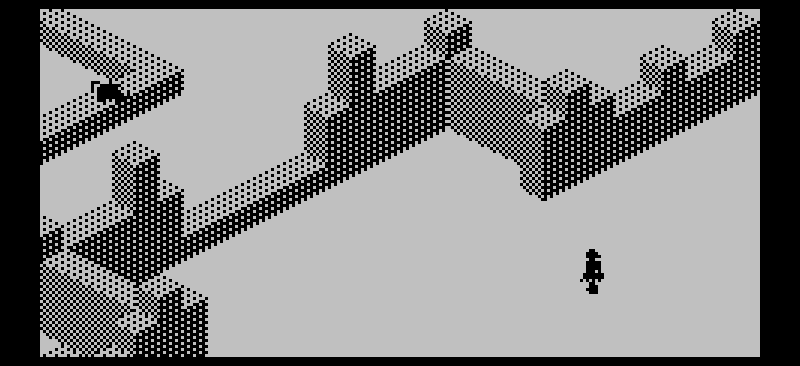
\includegraphics[width=0.7\textwidth]{ant-attack}
		\caption{Tela inicial de Ant Attack. Fonte: \cite{ant-attack}}\label{fig:ant_attack}
	\end{figure}
	\item[\textit{Knight Lore} (1984):] É um jogo de ação e aventura onde o jogador controla o herói
	\textit{Sabreman} (da série que começou com \textit{Sabre Wulf}), que foi mordido e amaldiçoado como lobisomem. Ele
	tem 40 dias para explorar um castelo de 128 salas, resolver quebra-cabeças e preparar um antídoto
	em um caldeirão. Foi um dos responsáveis por popularizar o gênero de aventura isométrica que por
	meio de sua técnica de mascaramento de imagem, chamada de \textit{Filmation}, permitia imagens passarem por
	baixo e por cima uma das outras sem que seus conteúdos colidissem, criando uma ilusão de profundidade
	que não era nativa dos computadores da época. O jogo foi publicado em 1984 e é considerado um trabalho
	seminal na história dos jogos britânicos, sendo coroado Jogo do Ano pela \textit{Golden Joystick Awards} e pela
	\textit{Popular Computing Weekly}, e lembrado como o primeiro jogo que ofereceu um mundo “explorável”, cuja
	influência persiste em jogos de RPG para computador.
	\begin{figure}[H]
		\centering
		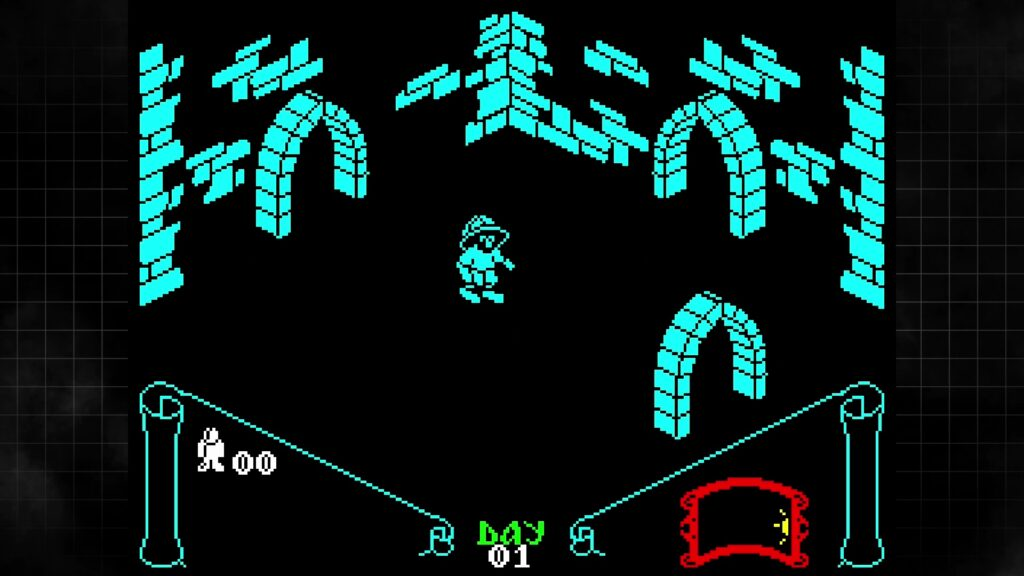
\includegraphics[width=0.7\textwidth]{knight-lore}
		\caption{Knight Lore. Fonte: \cite{knight-lore}}\label{fig:knight_lore}
	\end{figure}

\end{description}

No desenvolvimento moderno, a câmera isométrica é geralmente construída configurando-se
uma câmera 3D com projeção ortográfica alinhada a um ângulo fixo. Do ponto de vista de \textit{game design},
a adoção da câmera isométrica proporciona vantagens diretas para a jogabilidade e percepção do espaço, como:

\begin{description}
	\item[Clareza Espacial e Legibilidade:] Por não apresentar encurtamento perspectivo
	\mbox{(\textit{foreshortening})}, os objetos mantêm a mesma escala visual independentemente da sua
	distância em relação à câmera. Isso facilita a leitura imediata de distâncias, trajetórias e
	posições no cenário.
	\item[Ampla Visão do Cenário:] Permite que o jogador visualize simultaneamente o
	personagem principal, múltiplos inimigos ao redor e perigos do ambiente, favorecendo a
	antecipação de ações e o planejamento de reações.
	\item[Desempenho Visual Uniforme:] A ausência de cálculo de deformação de perspectiva
	simplifica o \textit{culling} de oclusão e otimiza a renderização de elementos estáticos e
	dinâmicos.

\end{description}

No entanto, o uso da isometria introduz desafios específicos que demandam soluções
intencionais de design, como a oclusão de elementos (quando objetos altos do cenário
escondem o personagem ou inimigos atrás deles) e a percepção de altura em saltos. Essas
particularidades exigem um planejamento de \textit{level design} e o uso de \textit{shaders} ou transparências
dinâmicas para preservar a orientação do jogador durante sua navegação pelo mapa. Diferentes jogos resolvem
problemas de isometria de maneiras distintas criativamente e tecnologicamente.

\begin{description}
	\item[Efeito Fantasma] Em jogos como Death's Door (2021) e Tunic (2022), quando o personagem passa atrás
	de uma árvore, parede ou ruína, o jogo utiliza um \textit{shader} de recorte ou transparência que
	desenha uma silhueta do personagem ``atrás'' do obstáculo. Assim, o jogador continua enxergando
	exatamente onde seu personagem está, mesmo com a geometria física bloqueando a visão direta.
	\begin{figure}[H]
		\centering
		\begin{subfigure}{0.48\textwidth}
			\centering
			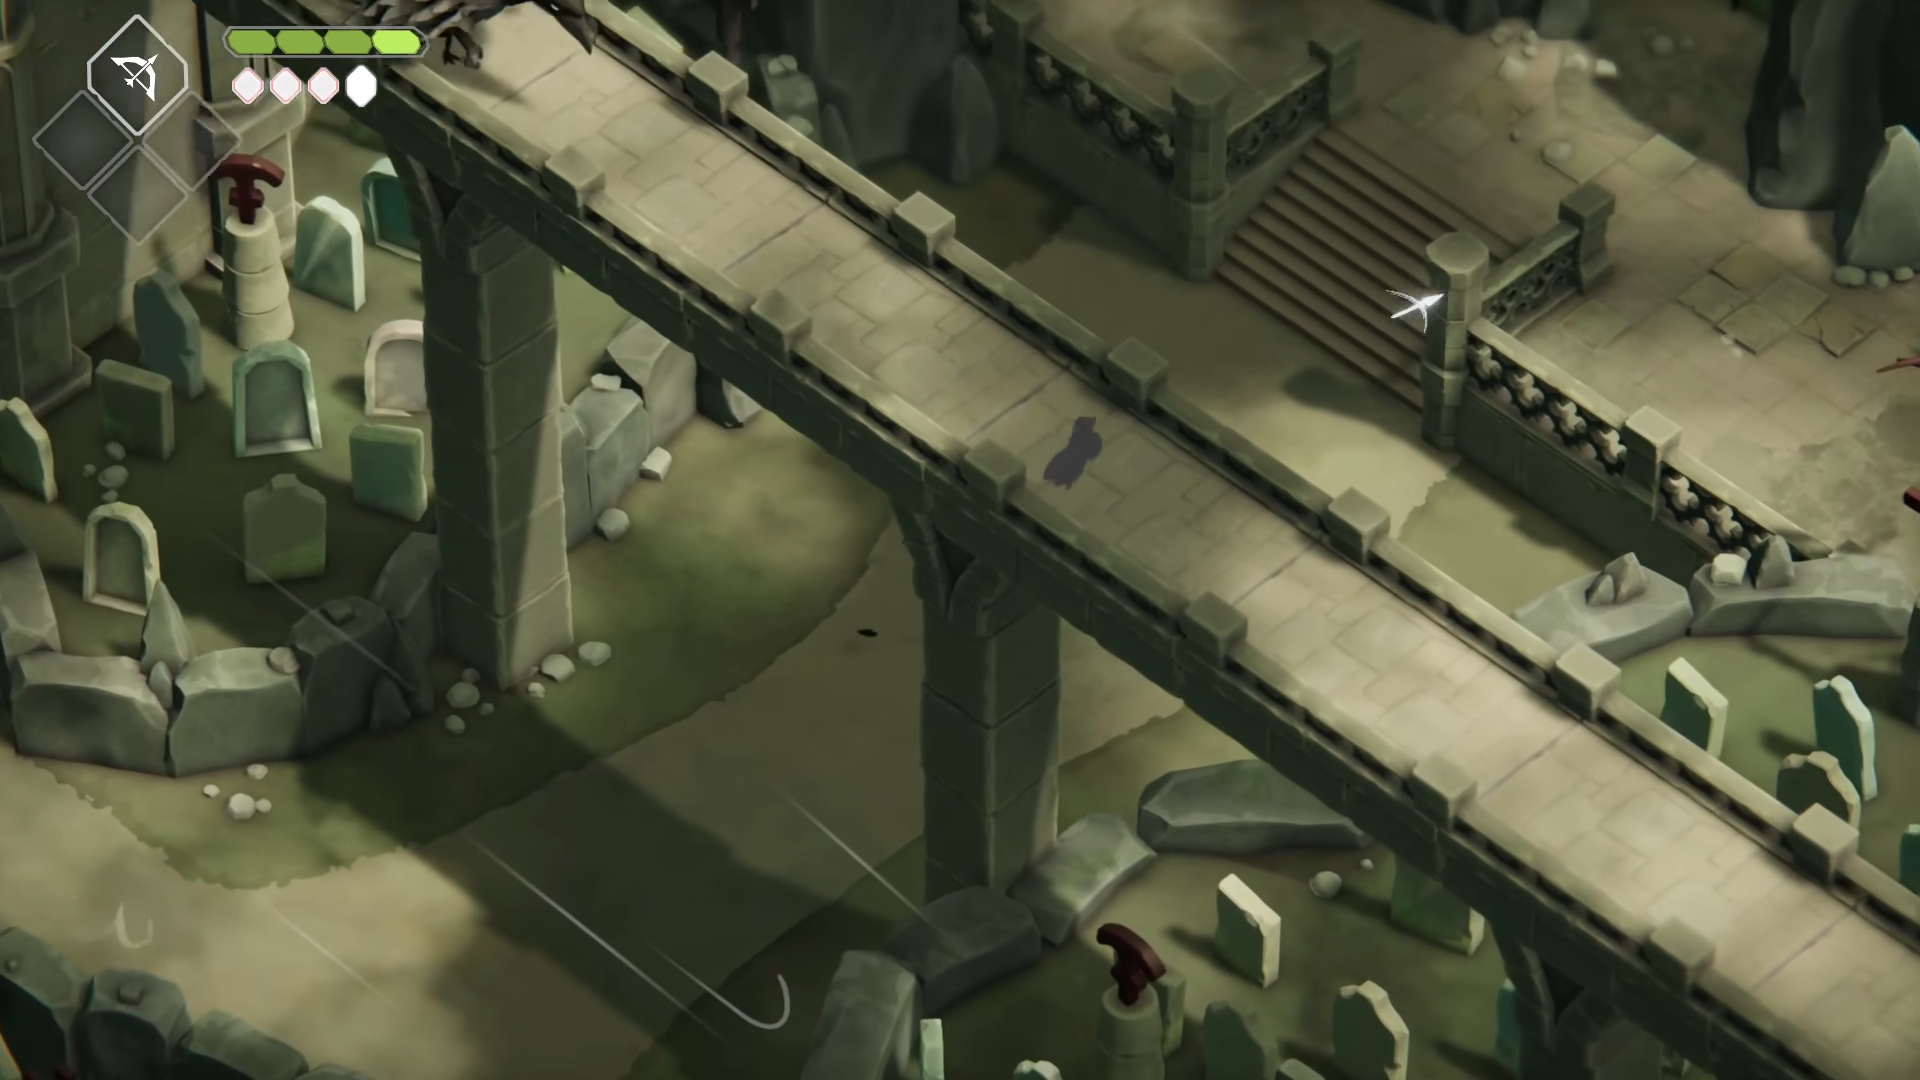
\includegraphics[width=\textwidth]{deaths_door_ghost}
			\caption{Death's Door (2021). Fonte: \cite{deaths-door-game}}\label{fig:ghost_effect_examples:deaths-door}
		\end{subfigure}
		\begin{subfigure}{0.48\textwidth}
			\centering
			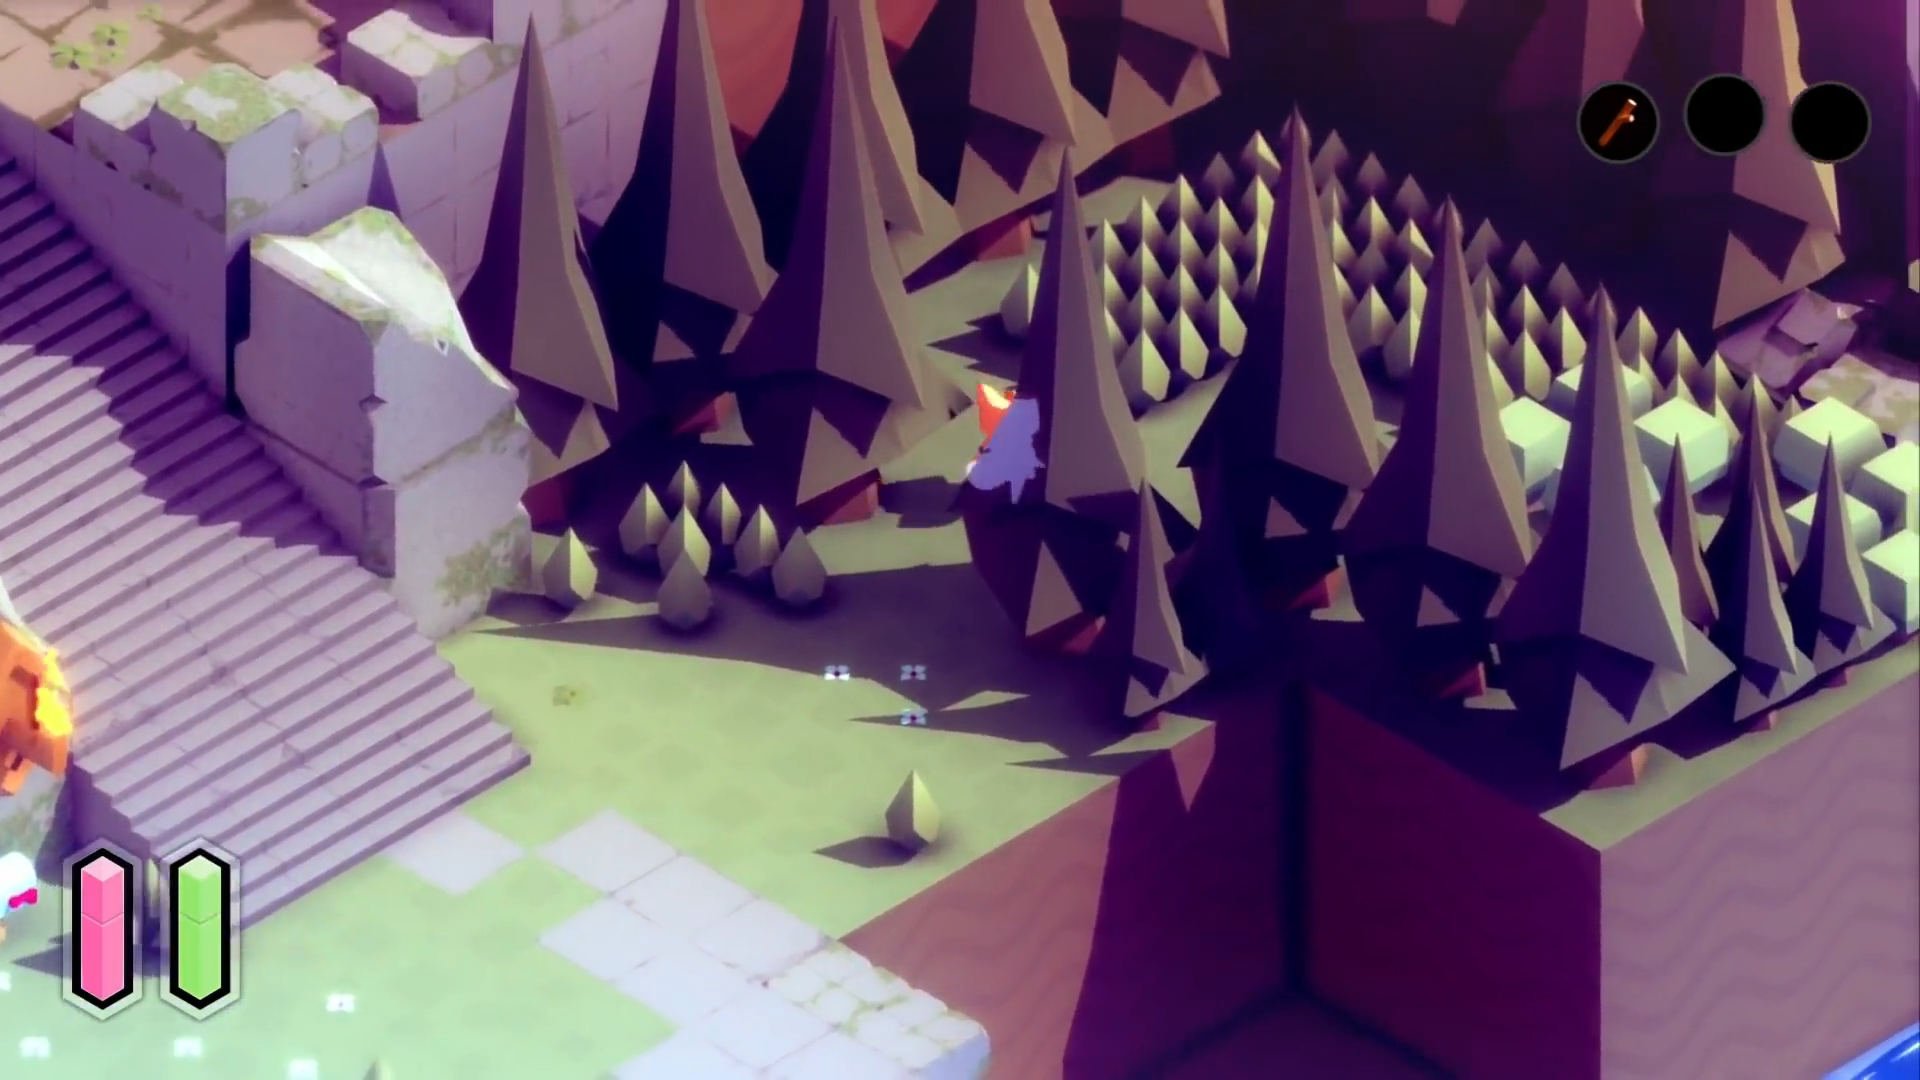
\includegraphics[width=\textwidth]{tunic_ghost}
			\caption{Tunic (2022). Fonte: \cite{tunic-game}}\label{fig:ghost_effect_examples:tunic}
		\end{subfigure}
		\caption{É possível ver a silhueta dos personagens através dos obstáculos.}\label{fig:ghost_effect_examples}
	\end{figure}

	\item[Transparência Dinâmica] Na presença de muitas paredes altas e masmorras como em Diablo IV (2023),
	quando o personagem se posiciona atrás de uma parede vertical em relação à câmera, um \textit{shader}
	de transparência acionado por \textit{raycasting}/linha de visão faz a parede desvanecer ou se dissolver
	completamente, revelando o espaço oculto.

	\begin{figure}[H]
		\centering
		\begin{subfigure}{0.48\textwidth}
			\centering
			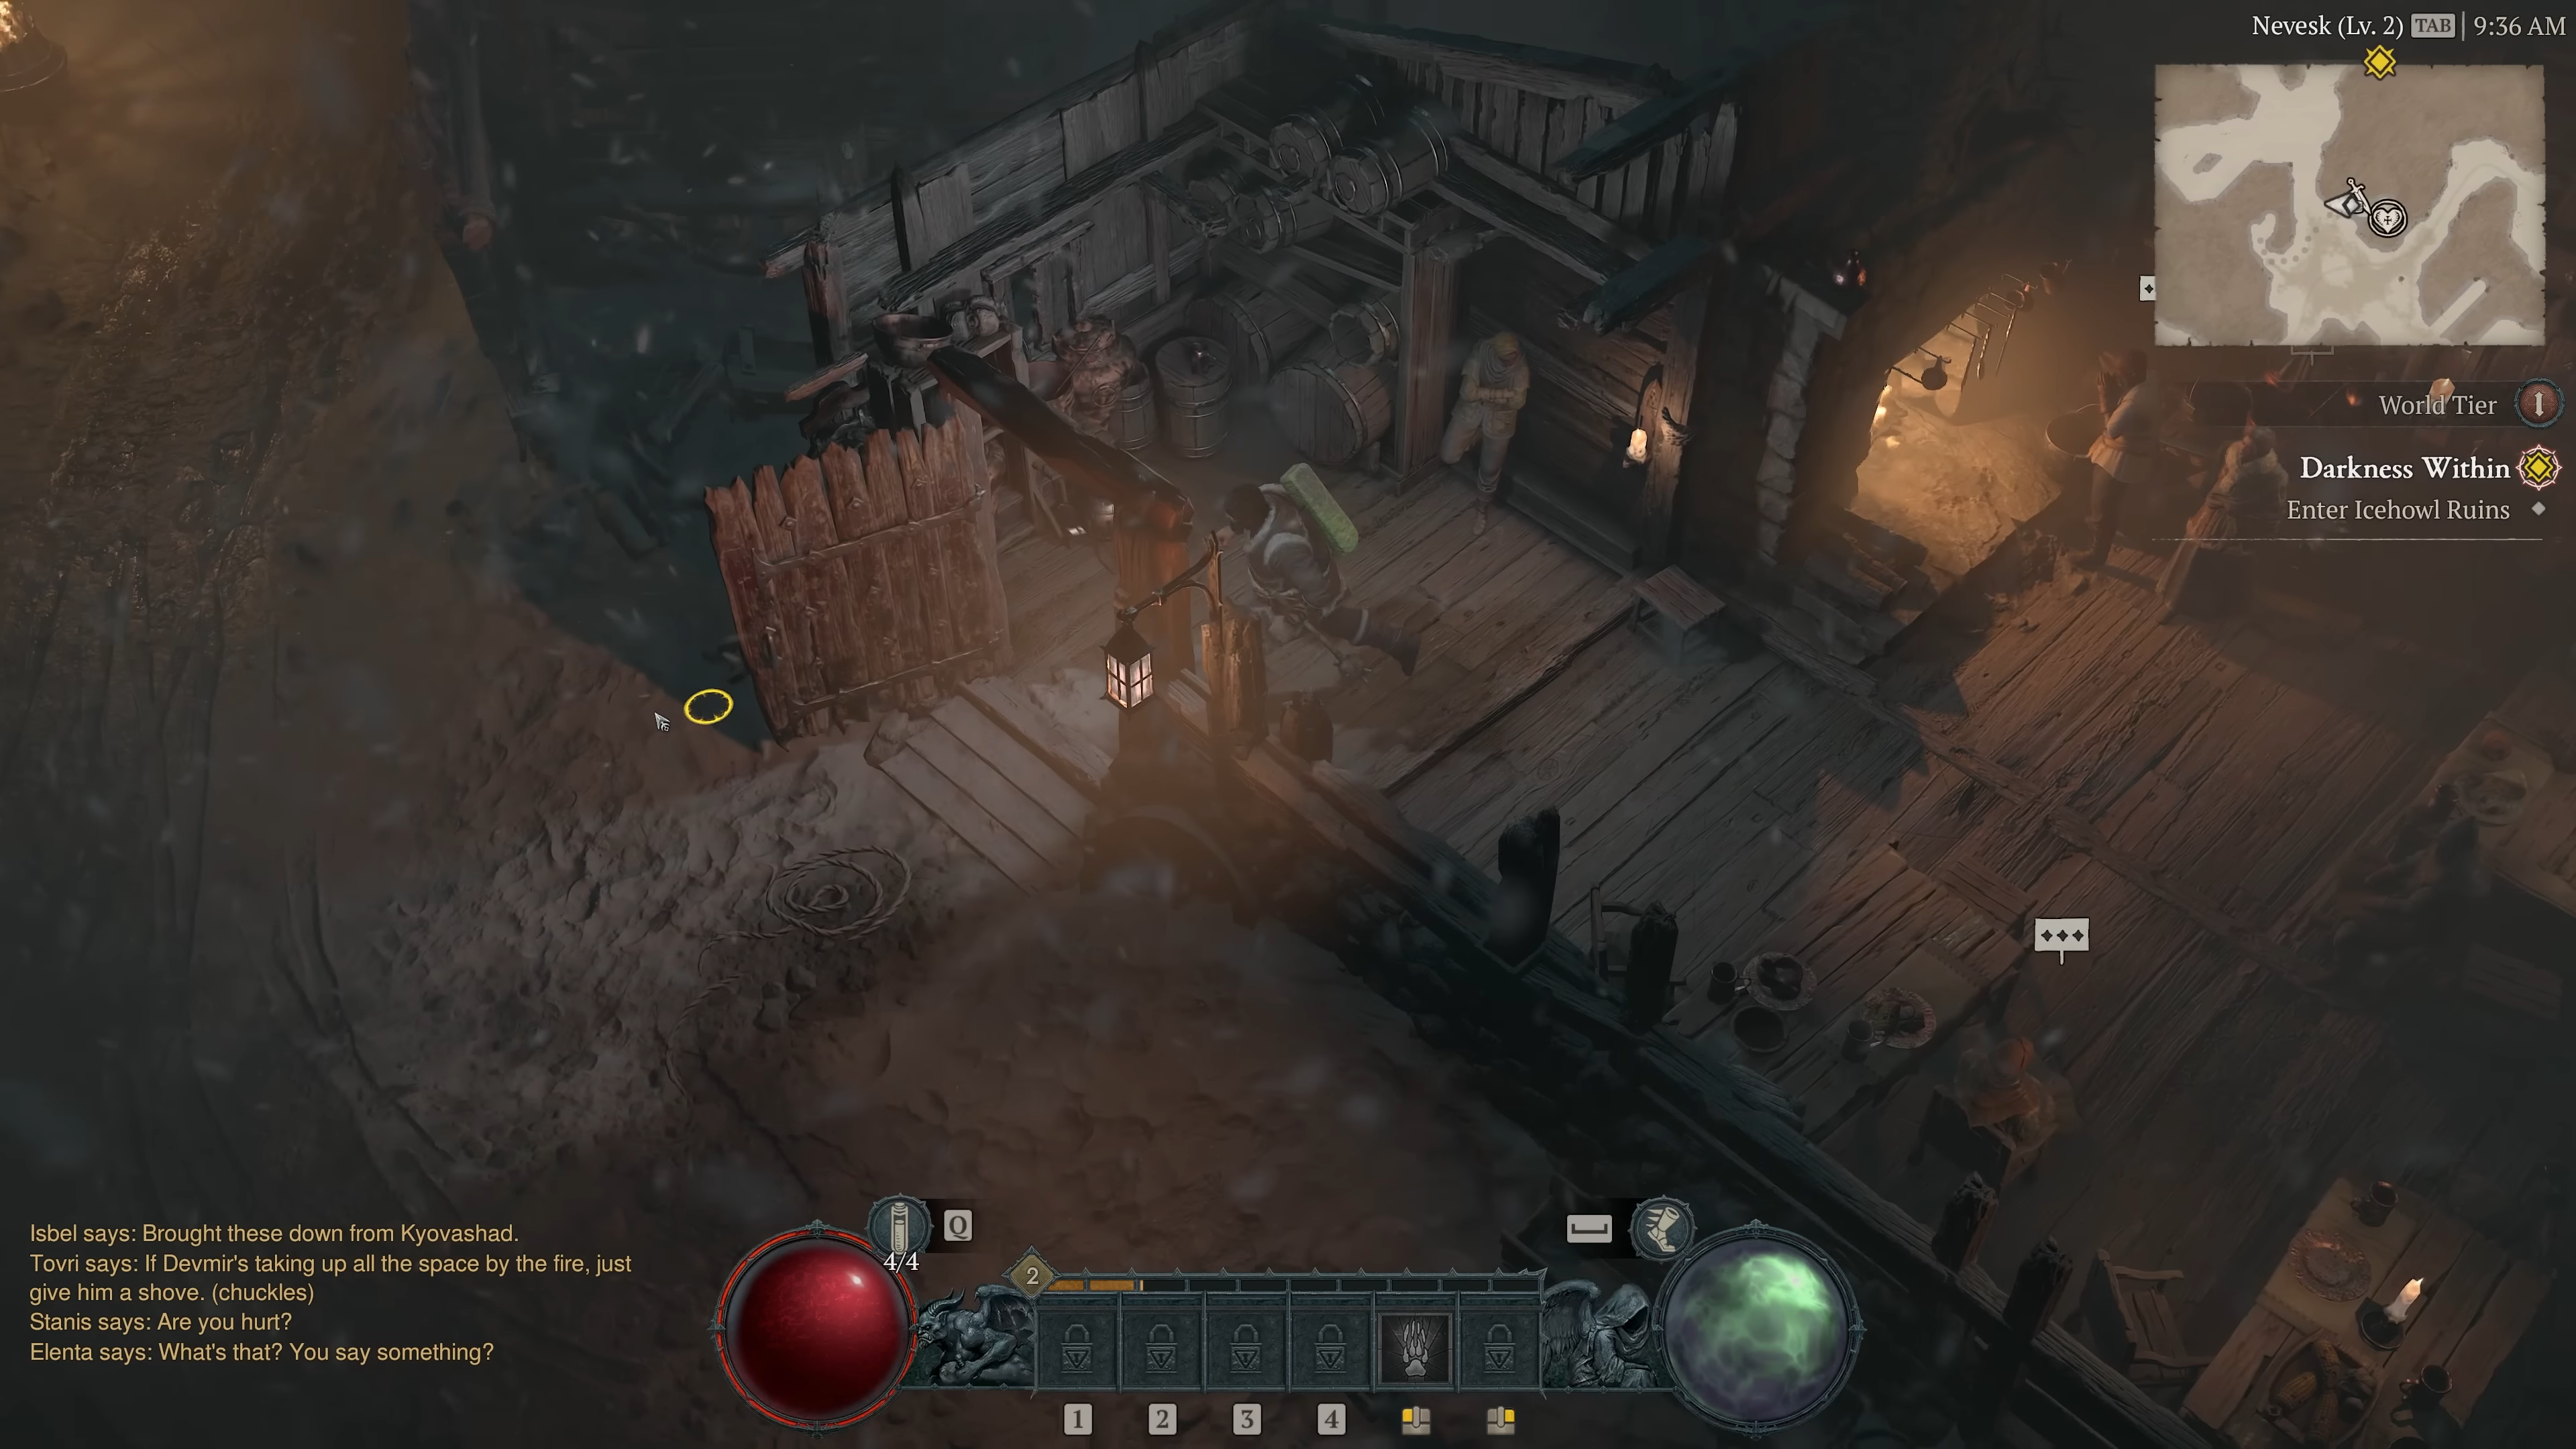
\includegraphics[width=\textwidth]{diablo_inside}
			\caption{Visão interna da casa.}\label{fig:fade_out_example:a}
		\end{subfigure}
		\begin{subfigure}{0.48\textwidth}
			\centering
			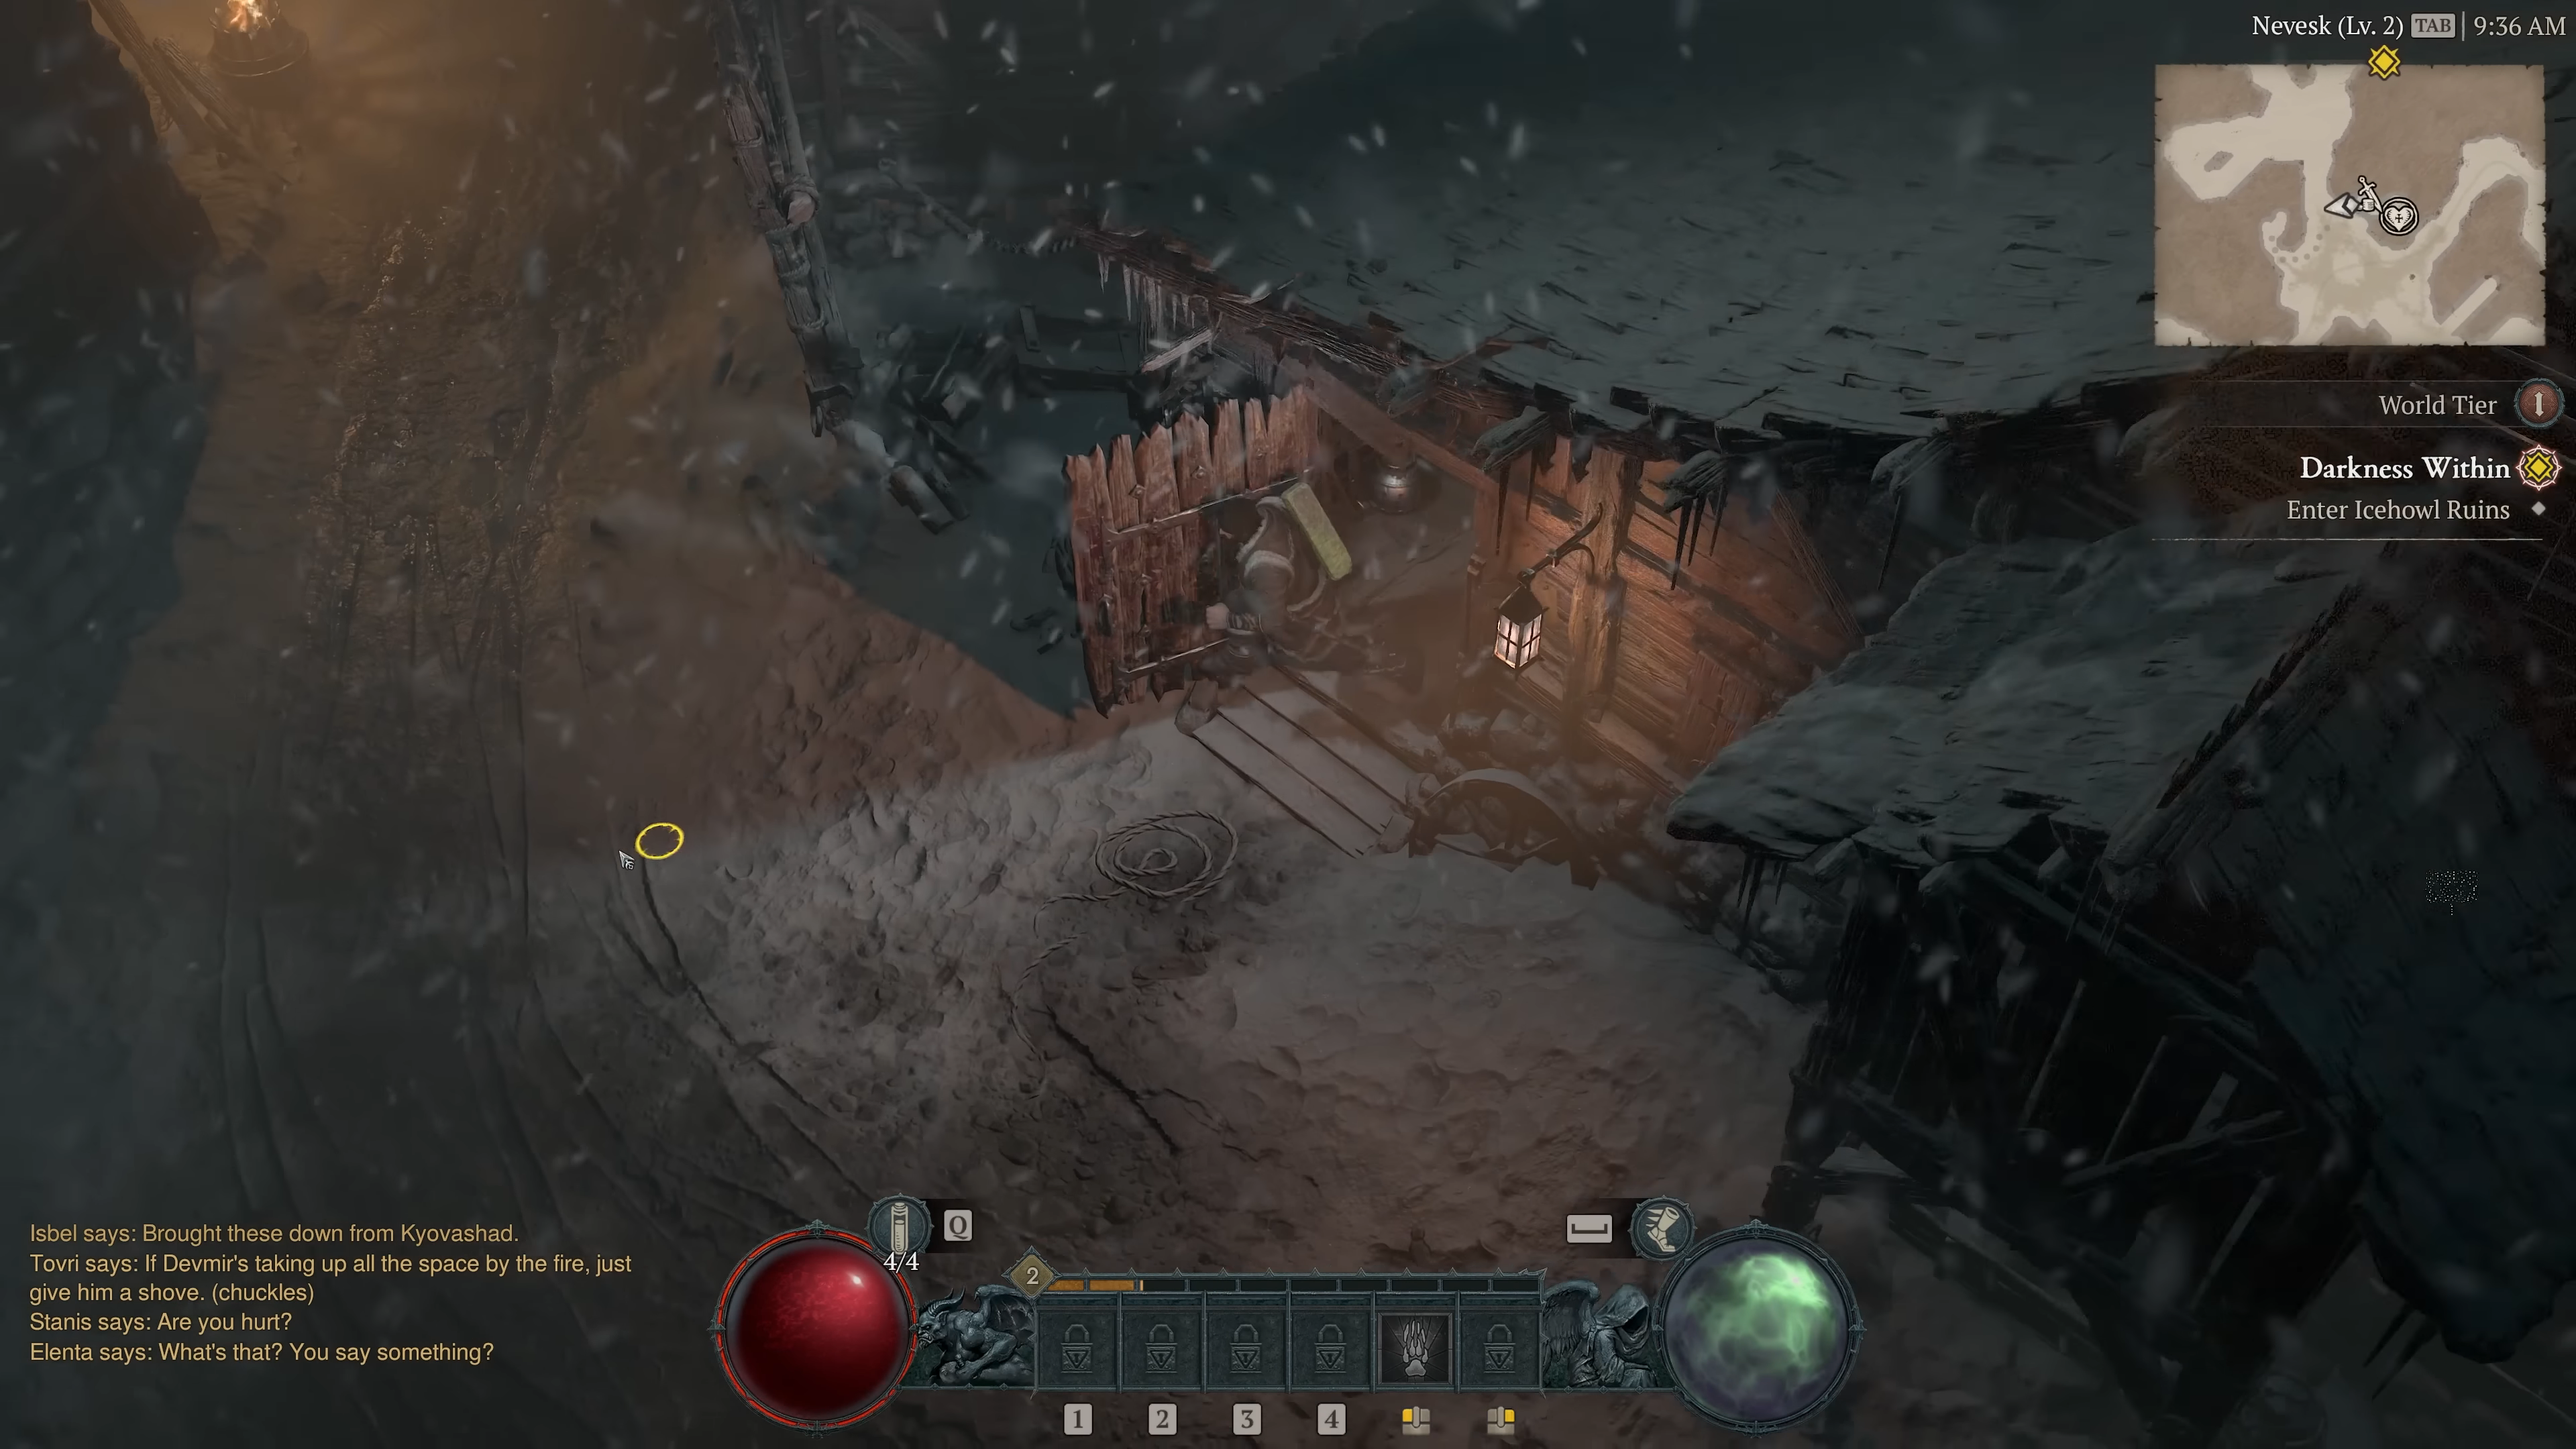
\includegraphics[width=\textwidth]{diablo_outside}
			\caption{Visão externa da casa.}\label{fig:fade_out_example:b}
		\end{subfigure}
		\caption{Transparência de obstáculos em Diablo IV (2023). Fonte: \cite{diablo-game}}\label{fig:fade_out_example}
	\end{figure}

	\item[Sombras de Queda] Os jogos isométricos utilizam da verticalidade para criar profundidade e
	complexidade espacial. Em jogos como Super Mario RPG (1996), a sombra do personagem não segue
	rigorosamente o ângulo da luz do sol do cenário. Em vez disso, há uma sombra projetada diretamente
	no plano do chão abaixo dele. Conforme o personagem pula, a sombra permanece estática no solo, e a
	distância entre o personagem e sua sombra indica visualmente a sua altura atual.

	\begin{figure}[H]
		\centering
		\begin{subfigure}{0.48\textwidth}
			\centering
			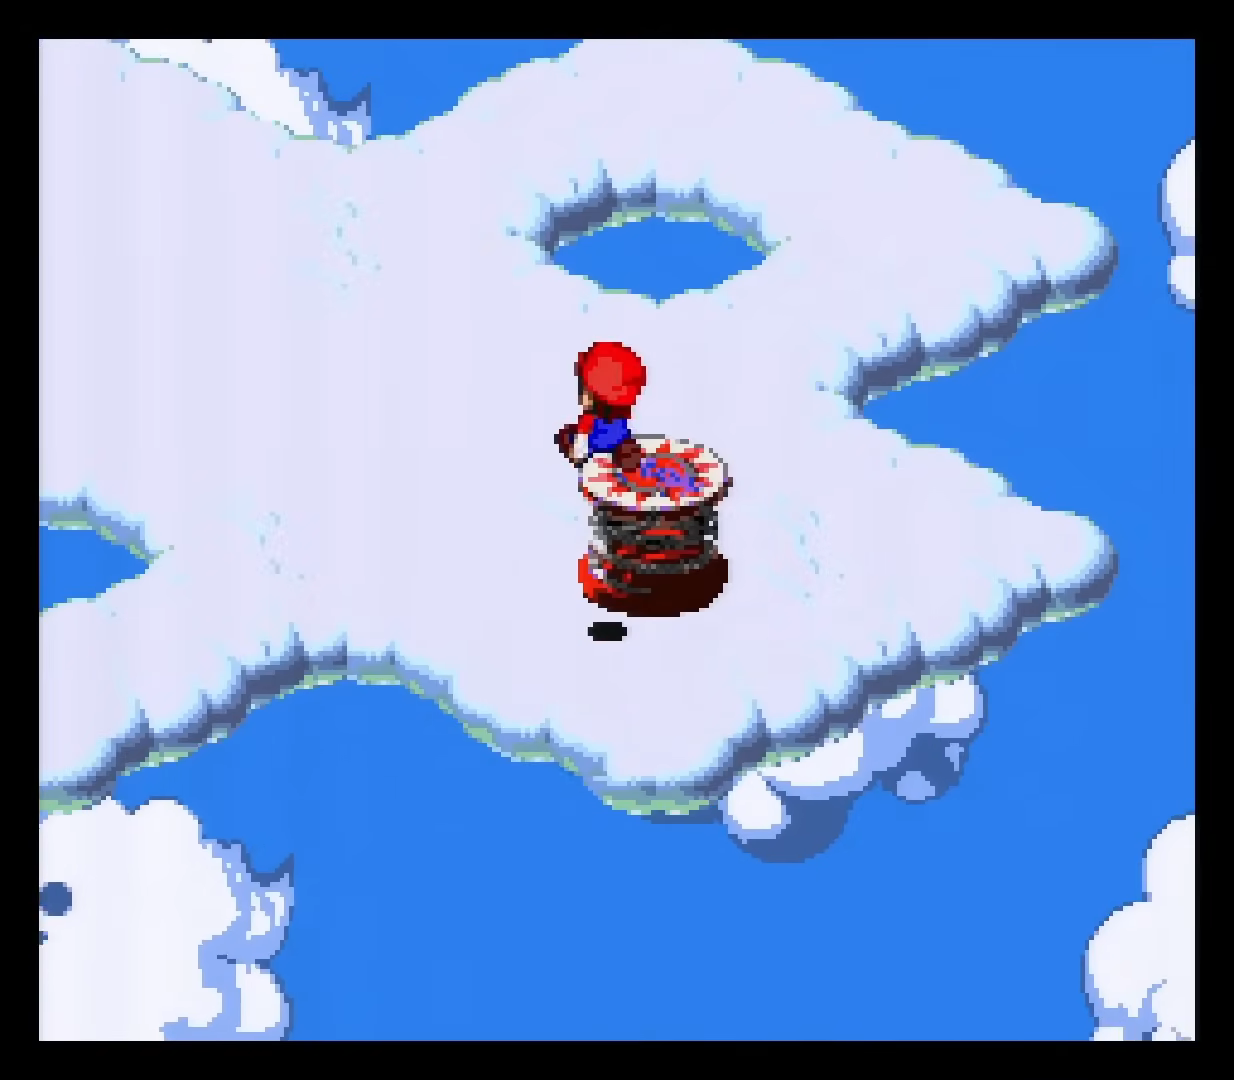
\includegraphics[width=\textwidth]{mario_distant}
			\caption{Personagem em posição elevada.}\label{fig:drop_shadow_example:a}
		\end{subfigure}
		\begin{subfigure}{0.48\textwidth}
			\centering
			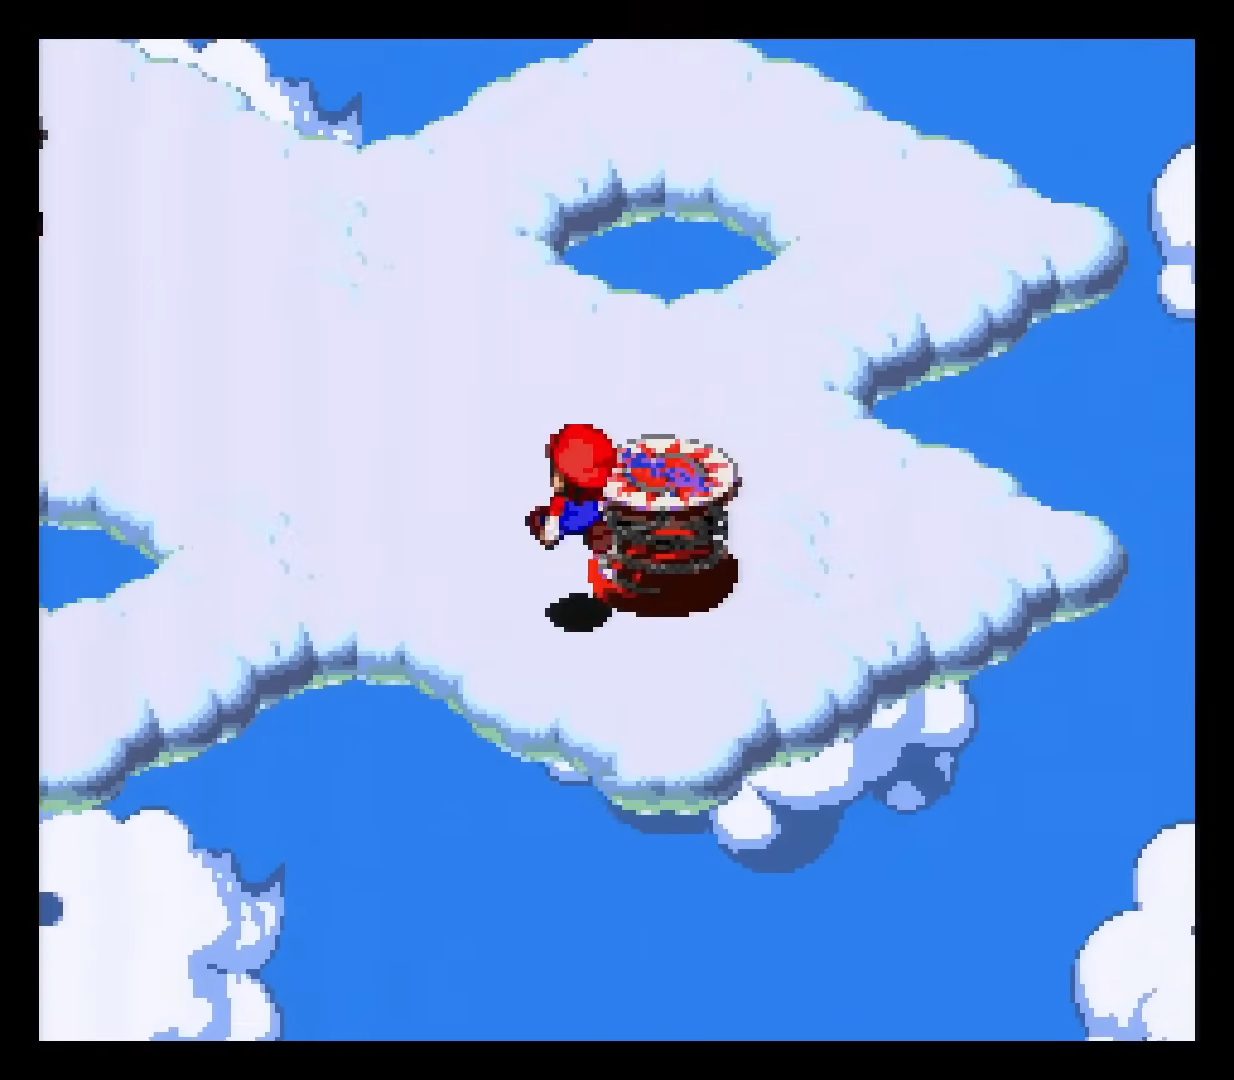
\includegraphics[width=\textwidth]{mario}
			\caption{Personagem em posição baixa.}\label{fig:drop_shadow_example:b}
		\end{subfigure}
		\caption{Sombra de queda em Super Mario RPG (1996). Fonte: \cite{mario-game}}\label{fig:drop_shadow_example}
	\end{figure}
\end{description}

\section{\textit{Low Poly}}
\label{sec:low_poly}

A identidade visual de um jogo 3D é fortemente influenciada pelo nível de detalhamento
geométrico de seus modelos. O termo \textit{low-poly} refere-se à prática de representar objetos
tridimensionais utilizando um número reduzido de polígonos (primariamente triângulos e
quadriláteros) em suas malhas poligonais (\textit{meshes}).

Do ponto de vista da computação gráfica, a redução da contagem de vértices e polígonos
diminui drasticamente o custo de processamento na etapa de transformação geométrica e
rasterização da GPU. Historicamente adotada como solução obrigatória para garantir taxas de
quadros aceitáveis em hardwares restritos, a modelagem \textit{low-poly} se tornou, eventualmente,
uma escolha artística comumente presente em jogos de desenvolvedores independentes devido a
sua simplicidade e eficiência.

Para efeitos comparativos, nos anos 1990 o Playstation 1 prometia a renderização de até 360.000
polígonos por segundo em testes de laboratório, mas na prática os jogos renderizavam entre 90.000 a
180.000 polígonos por segundo devido ao custo de processamento de texturas, shaders, etc. Nesta época,
um personagem costumava ter entre 400 a 800 polígonos dependendo de como o ambiente do jogo era
renderizado. A Lara Croft, protagonista do jogo \textit{Tomb Raider} (1996), possuía cerca de 250 polígonos em
seu modelo original.

\begin{figure}[H]
	\centering
	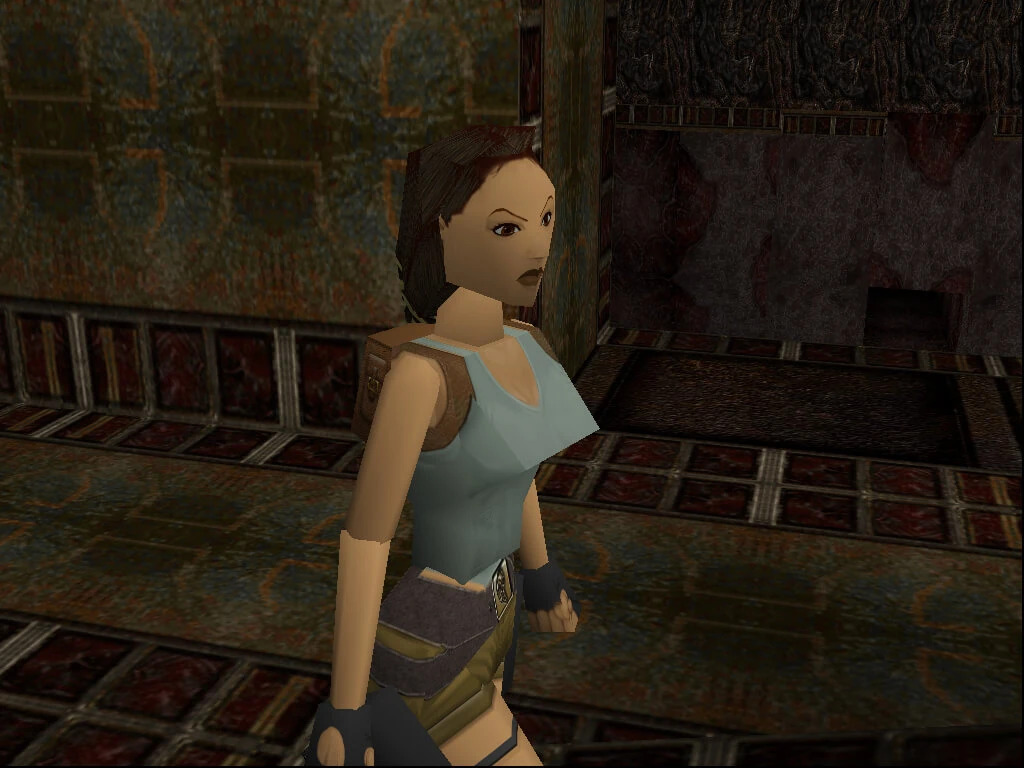
\includegraphics[width=0.6\textwidth]{tomb-raider-1996}
	\caption{Lara Croft (1996). Fonte: \cite{lara-croft-low}}\label{fig:lara_croft_low}
\end{figure}

Em \textit{Tomb Raider: Underworld} (2008), já no Playstation 3, a quantidade de polígonos em
seu modelo aumentou para 32,816, entrando para o \textit{Guinness World Records} como a personagem de video-game mais
detalhada da época.

\begin{figure}[H]
	\centering
	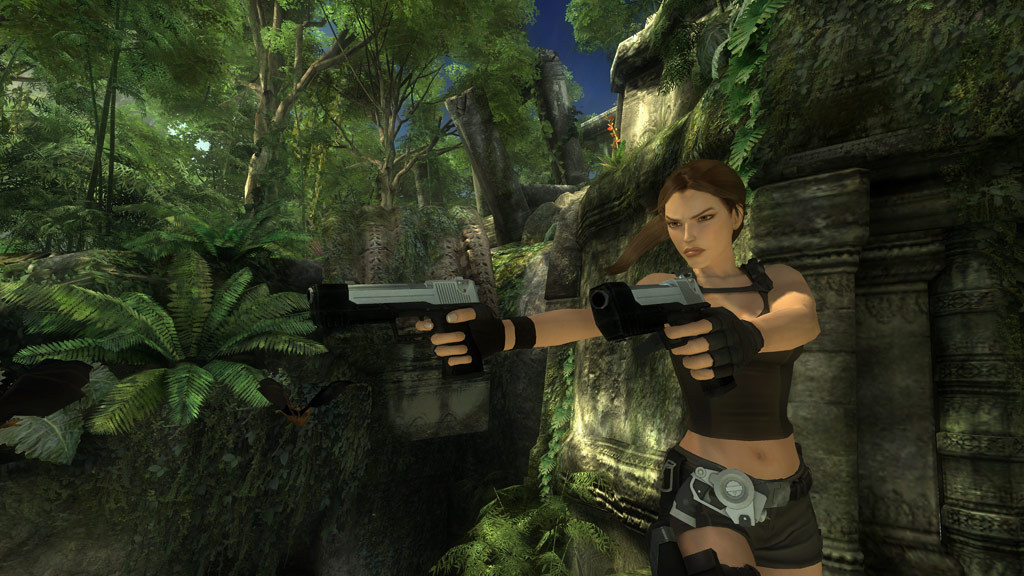
\includegraphics[width=0.6\textwidth]{tomb-raider-2008}
	\caption{Lara Croft (2008). Fonte: \cite{lara-croft-high}}\label{fig:lara_croft_high}
\end{figure}

Em 2017, Johan Lithvall compartilhou sobre sua participação no desenvolvimento do jogo
\textit{Horizon Zero Dawn} (2017) para Playstation 4, onde ficou encarregado do cabelo da protagonista
Aloy, e divulgou que ele possui cerca de 100.000 polígonos, mais que o triplo da quantidade de
um personagem inteiro de 2008.

\begin{figure}[H]
	\centering
	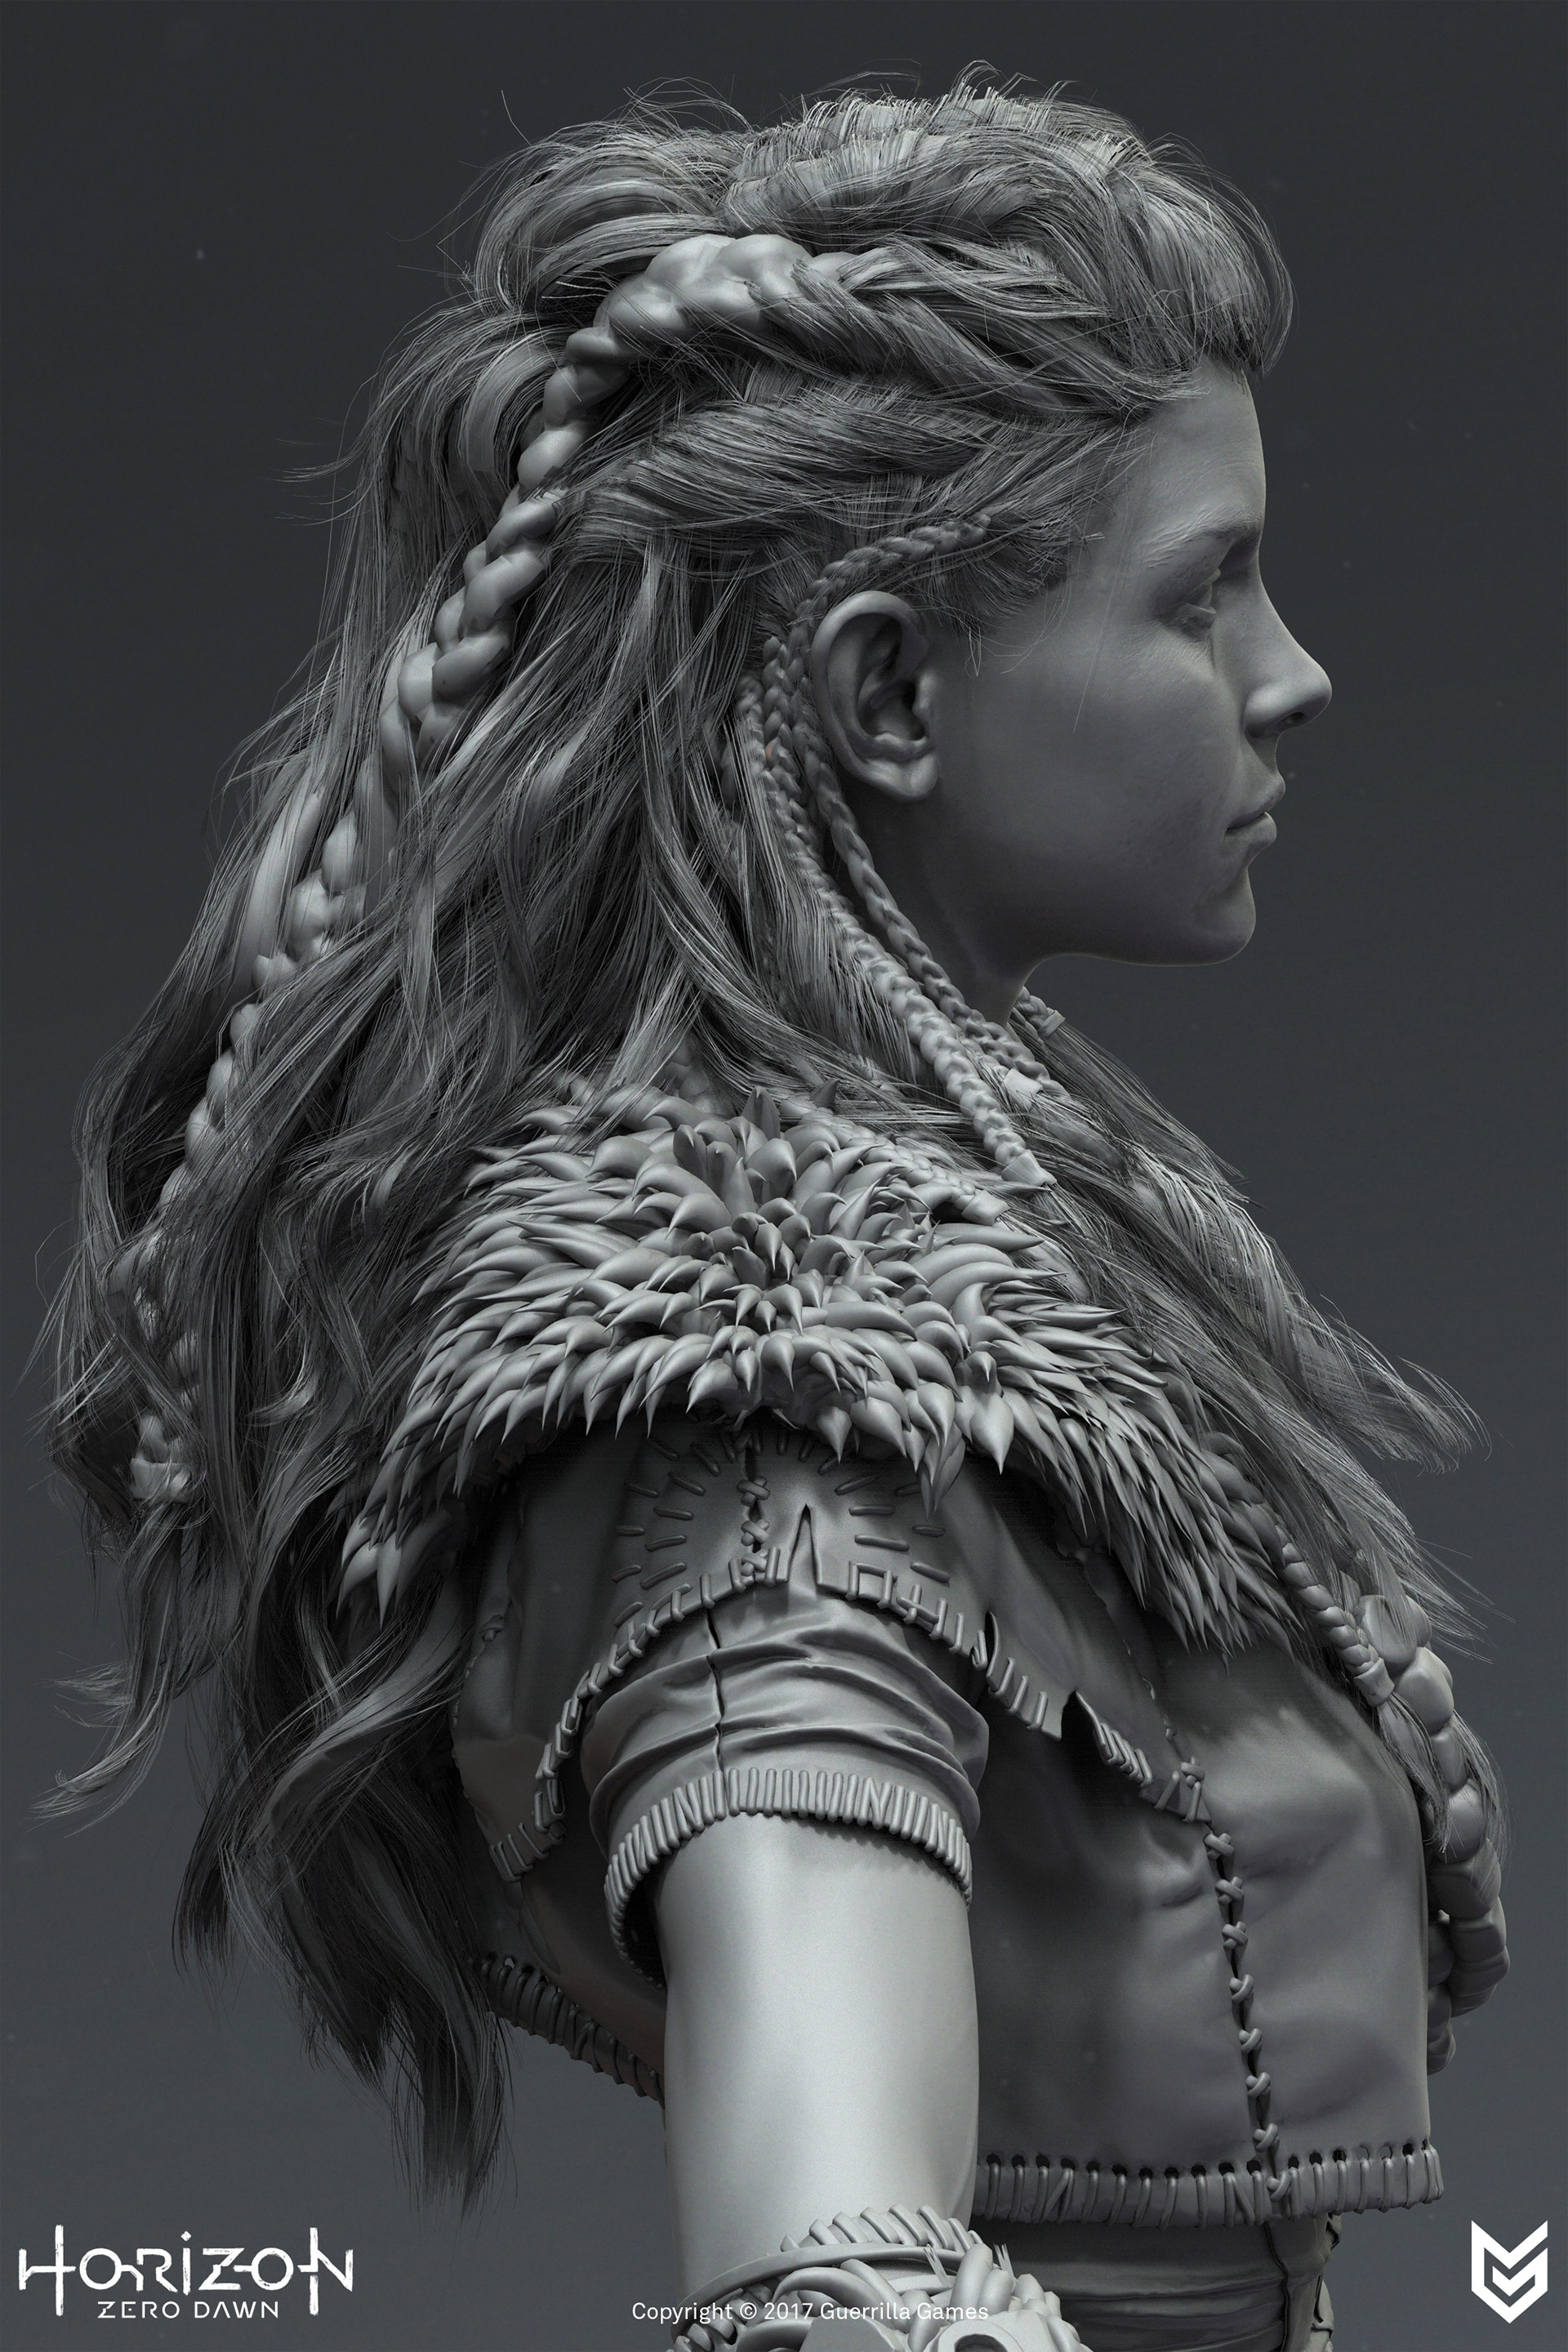
\includegraphics[width=0.3\textwidth]{aloy}
	\caption{Cabelo da Aloy (2017). Fonte: \cite{aloy}}\label{fig:aloy}
\end{figure}

Os modelos \textit{low poly} facilitam etapas do \textit{pipeline} de produção como Mapeamento UV
para as texturas, o \textit{rigging} (estruturação do esqueleto dos modelos), e animação.
pois com uma menor quantidade de polígonos, menor a necessidade de ponderações de peso, deformações
e poses extremamente complexas, simplificando os movimentos dos personagens.

No contexto artístico, o \textit{low-poly} se destaca por sua abstração geométrica, pois ao
dispensar texturas de alta resolução e malhas densas (\textit{high-poly}), os artistas utilizam
a própria estrutura dos polígonos para definir volumes, silhuetas e superfícies. Essa
abordagem é frequentemente combinada com técnicas de sombreamento plano (\textit{flat shading}),
onde as normais de iluminação são calculadas por face e não por vértice, acentuando as
arestas e proporcionando um aspecto visual limpo e estilizado.

Além disso, a união de modelos \textit{low-poly} com texturas pixelizadas (que é a proposta adotada neste
projeto) gera uma atmosfera estética que se assemelha aos jogos eletrônicos clássicos, reinterpretando-a
com ferramentas tridimensionais modernas. Essa linguagem visual não apenas reforça a legibilidade
espacial exigida por dinâmicas de jogo aceleradas, mas também reduz o consumo de memória de vídeo (VRAM),
permitindo que a capacidade de processamento seja direcionada para a estabilidade da física e para a
fluidez das interações no cenário.

\section{\textit{Fast-Paced}}
\label{sec:fast_paced}

Diferente de jogos focados em exploração de paisagens ou turnos estratégicos,
os jogos \textit{fast-paced} priorizam a velocidade e exigem do jogador respostas
motoras rápidas, reflexos apurados e tomadas de decisão instantâneas em meio a
sequências de ações.

Sob a ótica do \textit{game design}, o desenvolvimento de um jogo \textit{fast-paced} impõe
desafios à engenharia de movimentação e à arquitetura de colisão. Elementos como aceleração,
desaceleração, inércia e transições de animação precisam ser ajustados para eliminar qualquer
sensação de atraso (\textit{input lag} ou lentidão de resposta). O personagem deve responder
de forma imediata aos comandos do usuário, permitindo manobras fluidas como deslizes por
superfícies, saltos e desvios de projéteis.

Além disso, o ritmo do jogo está diretamente atrelado à clareza do \textit{level design}. Em cenários
dinâmicos, o jogador não pode perder tempo tentando entender o espaço ao seu redor. A arquitetura dos
mapas e os elementos visuais devem comunicar instantaneamente as rotas de fuga, os perigos e a posição
dos inimigos.

Assim, a combinação da estética \textit{low-poly} pixelizada e a projeção isométrica atuam de forma
sinergética com o gênero, pois ao remover ruídos visuais complexos e texturas fotorrealistas pesadas,
a cena torna-se limpa, garantindo a legibilidade espacial necessária para que o jogador possa agir e
reagir de forma fluida e sem comprometer o desempenho computacional.


%!TeX root=../main.tex

\chapter{Metodologia}
\label{cap:metodologia}

Devido a natureza do projeto em grupo, foram adotadas diversas convenções
de documentação, controle de versão e sistemas de gerenciamento para
conservar o fluxo de desenvolvimento.

\section{Projeto}
\label{sec:projeto}

O jogo foi desenvolvido utilizando o software Godot, que é uma ferramenta
de desenvolvimento de jogos. Foi utilizada sua própria linguagem (GDScript),
que é uma linguagem de alto-nível e orientada a objetos, com uma sintaxe
similar a python. O objetivo dessa linguagem é ser otimizada e fortemente
integrada à Godot Engine, permitindo maior flexibilidade de criação e integração.
Para manter o código-fonte organizado, e legível para todos os integrantes, foi
adotada a convenção de estilo oficial do GDScript, que pode ser encontrada em sua
documentação.



\section{Desenvolvimento}
\label{sec:desenvolvimento}


\section{Arquitetura}
\label{sec:arquitetura}

%!TeX root=../main.tex

\chapter{Proposta}
\label{cap:proposta}


\section{Câmera}
\label{sec:camera}

A visualização do ambiente de jogo adota uma perspectiva tridimensional com
projeção ortográfica, configurada sob uma inclinação espacial de estilo
isométrico, focando na legibilidade espacial dos cenários.

Para auxiliar nesta legibilidade, diferente de abordagens tradicionais com ângulos estáticos de visualização,
o sistema de câmera do projeto implementa um grau de liberdade de rotação
horizontal contínua em $360^\circ$ ao redor do personagem principal. Essa rotação
permite ao jogador girar o ponto de vista livremente para examinar cantos
ocultos do mapa, antecipar ameaças e navegar por rotas complexas sem
alterar a inclinação vertical fixa da projeção. Esta técnica é comumente
encontrada em CRPGs (\textit{Computer Role-Playing Games}) isométricos modernos, como \textit{Divinity: Original Sin 2} (\cite{original-sin}).

Para assegurar o ritmo acelerado (\textit{fast-paced}) da jogabilidade, o
acompanhamento da câmera em relação ao movimento do jogador é projetado
para ocorrer de forma suave (\textit{smooth follow}). Esse amortecimento visual
evita saltos bruscos resultantes de mudanças de direção repentinas do
personagem, mantendo a cena estável.

Por fim, o comportamento da câmera foi especificado para lidar com os
desafios de oclusão inerentes à perspectiva isométrica. Ao posicionar o
jogador atrás de estruturas altas ou elementos volumosos do cenário, a
câmera e os sistemas visuais integrados devem garantir a manutenção do
\textit{feedback} de localização do personagem, preservando a orientação espacial e
a fluidez dos comandos em qualquer direção do mapa.

\section{Movimentação}
\label{sec:movimentacao}

O sistema de locomoção do personagem principal foi estruturado para
atender aos requisitos de alta velocidade e resposta imediata inerentes do
gênero \textit{fast-paced}. O controle de deslocamento ocorre de maneira
omnidirecional no plano horizontal do cenário, permitindo ao jogador mover-se
fluidamente em qualquer direção independentemente da rotação atual da
câmera.

Para garantir o dinamismo exigido pelo projeto, o conjunto de ações
fundamentais de movimento é composto em:

\begin{description}
	\item[Deslocamento:] O personagem responde de forma
	contínua aos comandos direcionais.
	\item[Corrida:] O jogador dispõe de um estado de corrida
	que aumenta a sua velocidade de locomoção pelo mapa.
	\item[Pulo:] Mecânica de salto para permitir a navegação vertical
	sobre as plataformas sem quebrar o fluxo contínuo de movimento.
\end{description}

Do ponto de vista de \textit{game design}, as transições entre estados de movimento
(como a entrada e saída da corrida ou a execução de saltos) foram desenvolvidas
com foco na conservação de momento. Em vez de travamentos ou freadas abruptas,
o sistema de movimento preserva a energia cinética acumulada pelo jogador. Isto
permite, por exemplo, que a velocidade obtida durante uma corrida ou um deslize
seja transferida para o pulo. Essa continuidade física assegura que o jogador
mantenha total controle e fluidez ao se locomover pelo ambiente.


\section{Progressão e Mecânicas de Jogo}
\label{sec:progressao_e_mecanicas}


\section{Efeitos Visuais}
\label{sec:efeitos_visuais}


\section{Pós-processamento}
\label{sec:pos_processamento}


\section{Interação do Usuário}
\label{sec:interacao_usuario}


\section{Som}
\label{sec:som}


\section{Configurações}
\label{sec:configuracoes}
%!TeX root=../main.tex

\chapter{Entidades}
\label{cap:entidades}
%!TeX root=../main.tex

\chapter{Planos Futuros}
\label{cap:planos-futuros}
%!TeX root=../main.tex

\chapter{Conclusão}
\label{cap:conclusao}
\pagestyle{mainmatter}

%%%%%%%%%%%%%%% SEÇÕES FINAIS (BIBLIOGRAFIA E ÍNDICE REMISSIVO) %%%%%%%%%%%%%%%%
\backmatter

\pagestyle{backmatter}

% Espaço adicional no sumário antes das referências / índice remissivo
\addtocontents{toc}{\vspace{2\baselineskip plus .5\baselineskip minus .5\baselineskip}}

\printbibliography[
  title=\refname\label{sec:bib},
  heading=bibintoc,
]

\printindex

\end{document}